% Options for packages loaded elsewhere
%DIF LATEXDIFF DIFFERENCE FILE
%DIF DEL Epigenetics_Manuscript_submitted.tex   Wed Nov  2 12:18:44 2022
%DIF ADD Epigenetics_Manuscript.tex             Mon Feb 20 12:52:25 2023
\PassOptionsToPackage{unicode}{hyperref}
\PassOptionsToPackage{hyphens}{url}
%
\documentclass[
  11pt,
]{article}
\usepackage{lmodern}
\usepackage{amssymb,amsmath}
\usepackage{ifxetex,ifluatex}
\ifnum 0\ifxetex 1\fi\ifluatex 1\fi=0 % if pdftex
  \usepackage[T1]{fontenc}
  \usepackage[utf8]{inputenc}
  \usepackage{textcomp} % provide euro and other symbols
\else % if luatex or xetex
  \usepackage{unicode-math}
  \defaultfontfeatures{Scale=MatchLowercase}
  \defaultfontfeatures[\rmfamily]{Ligatures=TeX,Scale=1}
\fi
% Use upquote if available, for straight quotes in verbatim environments
\IfFileExists{upquote.sty}{\usepackage{upquote}}{}
\IfFileExists{microtype.sty}{% use microtype if available
  \usepackage[]{microtype}
  \UseMicrotypeSet[protrusion]{basicmath} % disable protrusion for tt fonts
}{}
\makeatletter
\@ifundefined{KOMAClassName}{% if non-KOMA class
  \IfFileExists{parskip.sty}{%
    \usepackage{parskip}
  }{% else
    \setlength{\parindent}{0pt}
    \setlength{\parskip}{6pt plus 2pt minus 1pt}}
}{% if KOMA class
  \KOMAoptions{parskip=half}}
\makeatother
\usepackage{xcolor}
\IfFileExists{xurl.sty}{\usepackage{xurl}}{} % add URL line breaks if available
\IfFileExists{bookmark.sty}{\usepackage{bookmark}}{\usepackage{hyperref}}
\hypersetup{
  pdftitle={Variation in histone configurations correlates with gene expression across nine inbred strains of mice},
  hidelinks,
  pdfcreator={LaTeX via pandoc}}
\urlstyle{same} % disable monospaced font for URLs
\usepackage[margin=1in]{geometry}
\usepackage{graphicx}
\makeatletter
\def\maxwidth{\ifdim\Gin@nat@width>\linewidth\linewidth\else\Gin@nat@width\fi}
\def\maxheight{\ifdim\Gin@nat@height>\textheight\textheight\else\Gin@nat@height\fi}
\makeatother
% Scale images if necessary, so that they will not overflow the page
% margins by default, and it is still possible to overwrite the defaults
% using explicit options in \includegraphics[width, height, ...]{}
\setkeys{Gin}{width=\maxwidth,height=\maxheight,keepaspectratio}
% Set default figure placement to htbp
\makeatletter
\def\fps@figure{htbp}
\makeatother
\setlength{\emergencystretch}{3em} % prevent overfull lines
\providecommand{\tightlist}{%
  \setlength{\itemsep}{0pt}\setlength{\parskip}{0pt}}
\setcounter{secnumdepth}{-\maxdimen} % remove section numbering

\newcommand{\beginsupplement}{%
        \setcounter{table}{0}
        \renewcommand{\thetable}{S\arabic{table}}%
        \setcounter{figure}{0}
        \renewcommand{\thefigure}{S\arabic{figure}}%
     }

\usepackage{natbib}

\usepackage{setspace} \doublespacing

\usepackage{fancyhdr}
\pagestyle{fancy}
\lhead{Tyler, Spruce, et al.}
\rhead{Epigenetic variation in nine inbred mouse strains}

\bibliographystyle{genome_research}
\ifluatex
  \usepackage{selnolig}  % disable illegal ligatures
\fi

\title{Variation in histone configurations correlates with gene
expression across nine inbred strains of mice}
\author{}
\date{\vspace{-2.5em}}
%DIF PREAMBLE EXTENSION ADDED BY LATEXDIFF
%DIF UNDERLINE PREAMBLE %DIF PREAMBLE
\RequirePackage[normalem]{ulem} %DIF PREAMBLE
\RequirePackage{color}\definecolor{RED}{rgb}{1,0,0}\definecolor{BLUE}{rgb}{0,0,1} %DIF PREAMBLE
\providecommand{\DIFaddtex}[1]{{\protect\color{blue}\uwave{#1}}} %DIF PREAMBLE
\providecommand{\DIFdeltex}[1]{{\protect\color{red}\sout{#1}}}                      %DIF PREAMBLE
%DIF SAFE PREAMBLE %DIF PREAMBLE
\providecommand{\DIFaddbegin}{} %DIF PREAMBLE
\providecommand{\DIFaddend}{} %DIF PREAMBLE
\providecommand{\DIFdelbegin}{} %DIF PREAMBLE
\providecommand{\DIFdelend}{} %DIF PREAMBLE
\providecommand{\DIFmodbegin}{} %DIF PREAMBLE
\providecommand{\DIFmodend}{} %DIF PREAMBLE
%DIF FLOATSAFE PREAMBLE %DIF PREAMBLE
\providecommand{\DIFaddFL}[1]{\DIFadd{#1}} %DIF PREAMBLE
\providecommand{\DIFdelFL}[1]{\DIFdel{#1}} %DIF PREAMBLE
\providecommand{\DIFaddbeginFL}{} %DIF PREAMBLE
\providecommand{\DIFaddendFL}{} %DIF PREAMBLE
\providecommand{\DIFdelbeginFL}{} %DIF PREAMBLE
\providecommand{\DIFdelendFL}{} %DIF PREAMBLE
%DIF HYPERREF PREAMBLE %DIF PREAMBLE
\providecommand{\DIFadd}[1]{\texorpdfstring{\DIFaddtex{#1}}{#1}} %DIF PREAMBLE
\providecommand{\DIFdel}[1]{\texorpdfstring{\DIFdeltex{#1}}{}} %DIF PREAMBLE
\newcommand{\DIFscaledelfig}{0.5}
%DIF HIGHLIGHTGRAPHICS PREAMBLE %DIF PREAMBLE
\RequirePackage{settobox} %DIF PREAMBLE
\RequirePackage{letltxmacro} %DIF PREAMBLE
\newsavebox{\DIFdelgraphicsbox} %DIF PREAMBLE
\newlength{\DIFdelgraphicswidth} %DIF PREAMBLE
\newlength{\DIFdelgraphicsheight} %DIF PREAMBLE
% store original definition of \includegraphics %DIF PREAMBLE
\LetLtxMacro{\DIFOincludegraphics}{\includegraphics} %DIF PREAMBLE
\newcommand{\DIFaddincludegraphics}[2][]{{\color{blue}\fbox{\DIFOincludegraphics[#1]{#2}}}} %DIF PREAMBLE
\newcommand{\DIFdelincludegraphics}[2][]{% %DIF PREAMBLE
\sbox{\DIFdelgraphicsbox}{\DIFOincludegraphics[#1]{#2}}% %DIF PREAMBLE
\settoboxwidth{\DIFdelgraphicswidth}{\DIFdelgraphicsbox} %DIF PREAMBLE
\settoboxtotalheight{\DIFdelgraphicsheight}{\DIFdelgraphicsbox} %DIF PREAMBLE
\scalebox{\DIFscaledelfig}{% %DIF PREAMBLE
\parbox[b]{\DIFdelgraphicswidth}{\usebox{\DIFdelgraphicsbox}\\[-\baselineskip] \rule{\DIFdelgraphicswidth}{0em}}\llap{\resizebox{\DIFdelgraphicswidth}{\DIFdelgraphicsheight}{% %DIF PREAMBLE
\setlength{\unitlength}{\DIFdelgraphicswidth}% %DIF PREAMBLE
\begin{picture}(1,1)% %DIF PREAMBLE
\thicklines\linethickness{2pt} %DIF PREAMBLE
{\color[rgb]{1,0,0}\put(0,0){\framebox(1,1){}}}% %DIF PREAMBLE
{\color[rgb]{1,0,0}\put(0,0){\line( 1,1){1}}}% %DIF PREAMBLE
{\color[rgb]{1,0,0}\put(0,1){\line(1,-1){1}}}% %DIF PREAMBLE
\end{picture}% %DIF PREAMBLE
}\hspace*{3pt}}} %DIF PREAMBLE
} %DIF PREAMBLE
\LetLtxMacro{\DIFOaddbegin}{\DIFaddbegin} %DIF PREAMBLE
\LetLtxMacro{\DIFOaddend}{\DIFaddend} %DIF PREAMBLE
\LetLtxMacro{\DIFOdelbegin}{\DIFdelbegin} %DIF PREAMBLE
\LetLtxMacro{\DIFOdelend}{\DIFdelend} %DIF PREAMBLE
\DeclareRobustCommand{\DIFaddbegin}{\DIFOaddbegin \let\includegraphics\DIFaddincludegraphics} %DIF PREAMBLE
\DeclareRobustCommand{\DIFaddend}{\DIFOaddend \let\includegraphics\DIFOincludegraphics} %DIF PREAMBLE
\DeclareRobustCommand{\DIFdelbegin}{\DIFOdelbegin \let\includegraphics\DIFdelincludegraphics} %DIF PREAMBLE
\DeclareRobustCommand{\DIFdelend}{\DIFOaddend \let\includegraphics\DIFOincludegraphics} %DIF PREAMBLE
\LetLtxMacro{\DIFOaddbeginFL}{\DIFaddbeginFL} %DIF PREAMBLE
\LetLtxMacro{\DIFOaddendFL}{\DIFaddendFL} %DIF PREAMBLE
\LetLtxMacro{\DIFOdelbeginFL}{\DIFdelbeginFL} %DIF PREAMBLE
\LetLtxMacro{\DIFOdelendFL}{\DIFdelendFL} %DIF PREAMBLE
\DeclareRobustCommand{\DIFaddbeginFL}{\DIFOaddbeginFL \let\includegraphics\DIFaddincludegraphics} %DIF PREAMBLE
\DeclareRobustCommand{\DIFaddendFL}{\DIFOaddendFL \let\includegraphics\DIFOincludegraphics} %DIF PREAMBLE
\DeclareRobustCommand{\DIFdelbeginFL}{\DIFOdelbeginFL \let\includegraphics\DIFdelincludegraphics} %DIF PREAMBLE
\DeclareRobustCommand{\DIFdelendFL}{\DIFOaddendFL \let\includegraphics\DIFOincludegraphics} %DIF PREAMBLE
%DIF LISTINGS PREAMBLE %DIF PREAMBLE
\RequirePackage{listings} %DIF PREAMBLE
\RequirePackage{color} %DIF PREAMBLE
\lstdefinelanguage{DIFcode}{ %DIF PREAMBLE
%DIF DIFCODE_UNDERLINE %DIF PREAMBLE
  moredelim=[il][\color{red}\sout]{\%DIF\ <\ }, %DIF PREAMBLE
  moredelim=[il][\color{blue}\uwave]{\%DIF\ >\ } %DIF PREAMBLE
} %DIF PREAMBLE
\lstdefinestyle{DIFverbatimstyle}{ %DIF PREAMBLE
	language=DIFcode, %DIF PREAMBLE
	basicstyle=\ttfamily, %DIF PREAMBLE
	columns=fullflexible, %DIF PREAMBLE
	keepspaces=true %DIF PREAMBLE
} %DIF PREAMBLE
\lstnewenvironment{DIFverbatim}{\lstset{style=DIFverbatimstyle}}{} %DIF PREAMBLE
\lstnewenvironment{DIFverbatim*}{\lstset{style=DIFverbatimstyle,showspaces=true}}{} %DIF PREAMBLE
%DIF END PREAMBLE EXTENSION ADDED BY LATEXDIFF

\begin{document}
\maketitle

Anna L. Tyler\textsuperscript{1,$*$}, Catrina
Spruce\textsuperscript{1,$*$}, Romy Kursawe\textsuperscript{2}, Annat
Haber\textsuperscript{2}, Robyn L. Ball\textsuperscript{1}, Wendy A.
Pitman\textsuperscript{1}, Alexander D. Fine\textsuperscript{1},
Narayanan Raghupathy\textsuperscript{1}, Michael
Walker\textsuperscript{1}, Vivek M. Philip\textsuperscript{1},
Christopher L. Baker\textsuperscript{1}, J. Matthew
Mahoney\textsuperscript{1}, Gary A. Churchill\textsuperscript{1},
Jennifer J. Trowbridge\textsuperscript{1}, Michael L.
Stitzel\textsuperscript{2}, Kenneth Paigen\textsuperscript{1}, Petko M.
Petkov\textsuperscript{1,$\dagger$}, Gregory W.
Carter\textsuperscript{1,$\dagger$}

\textsuperscript{1} The Jackson Laboratory for Mammalian Genetics, 600
Main St.~Bar Harbor, ME, 04609

\textsuperscript{2}The Jackson Laboratory for Genomic Medicine 299
Farmington Ave, Farmington, CT 06032

\(^*\) equal contribution \(^\dagger\) corresponding authors

Running title: Epigenetic variation in nine inbred mouse strains

\pagebreak

\hypertarget{abstract}{%
\section{Abstract}\label{abstract}}

\DIFdelbegin \DIFdel{It is well established that epigenetic features}\DIFdelend \DIFaddbegin \DIFadd{Epigenetic modifications}\DIFaddend , such as histone modifications and DNA
methylation, are \DIFdelbegin \DIFdel{associated with variation in gene expressionacross cell types . Less well known is
the extent to which
epigenetic states vary across
genetically diverse individuals, and
whether such variation corresponds to inter-individual }\DIFdelend \DIFaddbegin \DIFadd{important regulators of gene expression. Variation in
epigenetic modifications generates all the different cell types in a
multi-cellular organism from the same genome. Epigenetic variation is
also a critical component of variation in gene expression across
genetically distinct individuals. Understanding vraiation in phenotypes
across cell types and individuals requires an understanding of gene
regulation. Mice are a widely used model of health and disease in
humans, and in particular the diversity outbred (DO) mice and the inbred
founders that generated this population are widely used to dissect the
role of gene regulation in health and disease. Although there have been
many studies linking genetic variation to }\DIFaddend variation in gene expression
\DIFdelbegin \DIFdel{. To investigate genetically driven variation in epigenetics, we conducted a }\DIFdelend \DIFaddbegin \DIFadd{in this model, there is little known about how epigenetic modifications
vary in these strains. Mapping epigenetic modifications in this
population will improve our understanding of the mechanisms of gene
regulation in these widely used mice. To this end, we performed a strain
}\DIFaddend survey of epigenetic modifications \DIFdelbegin \DIFdel{and gene expression }\DIFdelend in hepatocytes of \DIFdelbegin \DIFdel{nine inbred mouse strains }\DIFdelend \DIFaddbegin \DIFadd{the DO founders. We
also surveyed DBA/2J, which with C57Bl/6J is one of the founders of the
BXD recombinant inbred strains of mice, another widely used population
in modeling disease}\DIFaddend . We surveyed four histone modifications (H3K4me1,
H3K4me3, H3K27me3, and H3K27ac), and DNA methylation. We used ChromHMM
to identify 14 chromatin states, each of which represented a distinct
combination of the four histone modifications. We found that\DIFdelbegin \DIFdel{chromatin states varied widely across the
nine strains and that epigenetic }\DIFdelend \DIFaddbegin \DIFadd{, in
contrast to DNA methylation, chromatin }\DIFaddend state was strongly correlated
with local gene expression \DIFdelbegin \DIFdel{. We replicated this correspondence between
}\DIFdelend \DIFaddbegin \DIFadd{across the inbred mice. We then imputed
}\DIFaddend chromatin state and \DIFdelbegin \DIFdel{gene expression in }\DIFdelend \DIFaddbegin \DIFadd{DNA methylation status into }\DIFaddend an independent
population of \DIFdelbegin \DIFdel{Diversity Outbred mice in which we imputed
local chromatin state . In
contrast, we found that DNA methylation did not vary across the inbred
strains and was not }\DIFdelend \DIFaddbegin \DIFadd{diversity outbred (DO) mice and found that imputed
chromatin state was more strongly }\DIFaddend correlated with variation in gene
expression \DIFdelbegin \DIFdel{in DO
mice. This work suggests that chromatin state is highly influenced by
local genotype and may be a primary mode through which expression }\DIFdelend \DIFaddbegin \DIFadd{than either DNA methylation status or local SNP genotype. We
use an example to illustrate how chromatin state can be aligned with
gene expression to identify specific genomic regions that may mediate
expression }\DIFaddend quantitative trait loci (eQTLs) \DIFdelbegin \DIFdel{are mediated. Through examples, we
demonstrate that naturally occurring }\DIFdelend \DIFaddbegin \DIFadd{through }\DIFaddend chromatin state
variation\DIFdelbegin \DIFdel{, in
conjunction with gene expression, can aid in functional annotation of
the mouse genome}\DIFdelend . Finally, we provide a data resource that documents
\DIFaddbegin \DIFadd{strain-specific }\DIFaddend variation in chromatin state in hepatocytes across \DIFdelbegin \DIFdel{genetically distinct
}\DIFdelend \DIFaddbegin \DIFadd{nine
widely used strains of laboratory }\DIFaddend mice.

\hypertarget{introduction}{%
\section{Introduction}\label{introduction}}

Although different cell types in an organism house the same genome, each
has a distinct pattern of gene expression. These cell-type specific
patterns of expression are established through epigenetic modification
of both histones \citep{pmid32671792, pmid29625185} and DNA methylation
\citep{pmid21701563, pmid20720541}, which influence the accessibility of
DNA to transcription machinery
\citep{lawrence2016lateral, jones2012functions, moore2013dna}.

This variation in epigenetic landscapes across cell types has been
extensively documented \citep{pmid21441907, pmid25693563} and has been
used to richly annotate functional elements in both mouse
\citep{stamatoyannopoulos2012encyclopedia, baker2019tissue, yue2014comparative}
and human genomes \citep{pmid25693563, pmid23595227, pmid20657582}. Such
functional annotations provide insight into mechanisms of gene
regulation. Because the majority of disease-associated genetic variants
discovered in humans are in gene regulatory regions, it has been
suggested that it is the regulation of gene expression, rather than
alteration of protein function, that is the primary mechanism through
which genetic variation confers disease risk
\citep{maurano2012systematic, farh2015genetic, pmid21617055, pmid19474294}.
Detailed epigenomic landscapes, therefore, may provide important
mechanistic insight linking genotype to disease risk.

\DIFdelbegin \DIFdel{However, although variation in epigenetic modifications across cell
types has been deeply explored, we have
relatively little knowledge of
inter-individual variation in epigenetic modifications. Does }\DIFdelend \DIFaddbegin \DIFadd{Work in humans \mbox{%DIFAUXCMD
\citep{mcvicker2013identification, kang2021genetic}}\hspace{0pt}%DIFAUXCMD
, rats
\mbox{%DIFAUXCMD
\citep{rintisch2014natural}}\hspace{0pt}%DIFAUXCMD
, and cattle \mbox{%DIFAUXCMD
\citep{prowse2022genetic} }\hspace{0pt}%DIFAUXCMD
have
linked }\DIFaddend genetic variation across individuals \DIFdelbegin \DIFdel{influence the epigenetic landscape? To what
extent does this variation result in altered gene expression ? The
generation of a more complete picture of inter-individual variation in epigenetic modifications will increase our understanding of the }\DIFdelend \DIFaddbegin \DIFadd{to variation in the histone
landscape. Such variation can alter gene regulation through the
disruption of transcription factor binding sites and other mechanisms
\mbox{%DIFAUXCMD
\citep{mcvicker2013identification}}\hspace{0pt}%DIFAUXCMD
. In support of this idea, genetic
loci associated with variability in the histone landscape frequently
overlap with expression quantitative trait loci (eQTL)
\mbox{%DIFAUXCMD
\citep{kang2021genetic, 
rintisch2014natural, prowse2022genetic} }\hspace{0pt}%DIFAUXCMD
and genetic loci associated with
clinical outcomes \mbox{%DIFAUXCMD
\citep{kang2021genetic}}\hspace{0pt}%DIFAUXCMD
. For example, genetic variants
in the promoters of CAPN1 and LINC00959 which were associated with
variation in H3K4me3 and H3K27ac modifications, were also associated
with variation in expression of the locally encoded genes and with
patient outcomes following surgery for lung adenocarcenoma
\mbox{%DIFAUXCMD
\citet{kang2021genetic}}\hspace{0pt}%DIFAUXCMD
. Similarly, studies have identified genetic loci
that are associated both with variation in DNA methylation and higher
level clinical outcomes such as immune dysregulation and asthma
\mbox{%DIFAUXCMD
\citep{hawe2022genetic}}\hspace{0pt}%DIFAUXCMD
.
}

\DIFadd{This body of work demonstrates the important links between genetic
variation, epigenetic variation, and higher level phenotypes. Thus,
mapping variation of the epigenetic landscape in models of human disease
is critical to understanding }\DIFaddend mechanisms of gene regulation \DIFdelbegin \DIFdel{, provide insights into the mechanisms
establishing cell type-specific epigenetic landscapes, and improve the functional annotation of the genome as it relates to the regulation of gene expression and disease risk.
}\DIFdelend \DIFaddbegin \DIFadd{in these
models. Laboratory mice are one of the most widely used models of human
disease, and yet there is little known about the landscape of epigenetic
modifications in these animals.
}\DIFaddend 

\DIFdelbegin \DIFdel{To investigate the
effect of genetic
variation on epigenetic variation, we performed a }\DIFdelend \DIFaddbegin \DIFadd{In the last decades the development of the diversity outbred (DO) mice
\mbox{%DIFAUXCMD
\citep{Svenson:2012hq, churchill2012diversity, 
koyuncu2021cxcl1, kurtz2020diversity, bogue2015collaborative, 
kebede2014insights, keller2019gene} }\hspace{0pt}%DIFAUXCMD
and their sister population, the
collaborative cross (CC) mice \mbox{%DIFAUXCMD
\citep{threadgill2011collaborative, 
threadgill2012ten, durrant2011collaborative, mao2015identification, 
graham2021baseline}}\hspace{0pt}%DIFAUXCMD
, has demonstrated the critical importance of genetic
diversity in our understanding of disease biology. However, the
epigenetic landscape in these important models is still relatively
unexplored. To address this gap in knowledge, we undertook a strain
}\DIFaddend survey of epigenetic variation in hepatocytes across \DIFdelbegin \DIFdel{nine
inbred mouse strains. We included }\DIFdelend the eight founders
of the \DIFdelbegin \DIFdel{Diversity
Outbred/Collaborative Cross (}\DIFdelend DO/CC \DIFdelbegin \DIFdel{) \mbox{%DIFAUXCMD
\citep{Svenson:2012hq} }\hspace{0pt}%DIFAUXCMD
}\DIFdelend mice, as well as DBA/2J, which, along with C57BL/6J, is one
of the founders of the widely used BxD recombinant inbred panel of mice
\citep{Ashbrook:2019bd}. We assayed four histone modifications: H3K4me3,
which is associated with promoter regions
\citep{heintzman2007distinct, pmid15680324}, H3K4me1, which is
associated with enhancer regions \citep{heintzman2007distinct},
H3K27me3, which is associated with polycomb repression
\citep{bonasio2010molecular}, and H3K27ac, which has been associated
with enhancement of active enhancers and promoters
\citep{creyghton2010histone, heintzman2009histone, rada2011unique}. We
also assayed DNA methylation which is associated with \DIFdelbegin \DIFdel{repression of
expression \mbox{%DIFAUXCMD
\citep{moore2013dna, jones2012functions}}\hspace{0pt}%DIFAUXCMD
.
}\DIFdelend \DIFaddbegin \DIFadd{variation in gene
expression depending on its position relative to the gene
\mbox{%DIFAUXCMD
\citep{moore2013dna, jones2012functions}}\hspace{0pt}%DIFAUXCMD
. Methylation of DNA in
promoters reduces gene expression, whereas methylation of DNA in
insulators reduces the effect of the insulator thereby increasing
expression of the targeted gene \mbox{%DIFAUXCMD
\citep{jones2012functions}}\hspace{0pt}%DIFAUXCMD
.
}\DIFaddend 

We used ChromHMM \citep{Ernst:2012ii} to identify 14 chromatin states,
each representing a unique combination of the four histone marks. We
investigated the association between variation in these states and
variation in gene expression across the nine strains. We \DIFdelbegin \DIFdel{separately
}\DIFdelend \DIFaddbegin \DIFadd{also
}\DIFaddend investigated the relationship between DNA methylation and gene
expression across strains.

We further investigated the relationship between epigenetic state and
\DIFaddbegin \DIFadd{local regulation of }\DIFaddend gene expression by imputing the 14 chromatin states
and DNA methylation into a population of DO mice. We then mapped gene
expression to the imputed epigenetic states to assess the extent to
which \DIFdelbegin \DIFdel{eQTLs were
driven by }\DIFdelend \DIFaddbegin \DIFadd{expression quantitative trait loci (eQTLs) in the DO were related
to }\DIFaddend variation in epigenetic \DIFdelbegin \DIFdel{modification}\DIFdelend \DIFaddbegin \DIFadd{modifications}\DIFaddend .

\hypertarget{results}{%
\section{Results}\label{results}}

Both gene expression and epigenetic state were consistent within mouse
strains but varied across the strains suggesting strong genetic
regulation of both modalities. This is seen as a clustering of
individuals from the same strain in principal component plots of
transcriptomic and epigenetic features (\DIFdelbegin \DIFdel{Figure }\DIFdelend \DIFaddbegin \DIFadd{Fig. }\DIFaddend \ref{fig:pc_plots}).
Patterns of gene expression (\DIFdelbegin \DIFdel{Figure }\DIFdelend \DIFaddbegin \DIFadd{Fig. }\DIFaddend \ref{fig:pc_plots}A), DNA methylation
(\DIFdelbegin \DIFdel{Figure }\DIFdelend \DIFaddbegin \DIFadd{Fig. }\DIFaddend \ref{fig:pc_plots}B) and individual histone modifications (\DIFdelbegin \DIFdel{Figure }\DIFdelend \DIFaddbegin \DIFadd{Fig.
}\DIFaddend \ref{fig:pc_plots}C-F) clustered in similar patterns although a
relatively small percent of the variation in the methylome was related
to strain. The three subspecies \textit{musculus} (in red),
\textit{castaneous} (in green) and \textit{domesticus} (all others) were
widely separated suggesting that subspecies structure made up the
majority of the observed variance. The \text{domesticus} strains largely
clustered together. These data provide evidence that epigenetic features
relate to gene expression in a manner that is consistent with the
subspecific origin of the mouse strains \DIFdelbegin \DIFdel{.
}\DIFdelend \DIFaddbegin \DIFadd{\mbox{%DIFAUXCMD
\citep{yang2007subspecific}}\hspace{0pt}%DIFAUXCMD
. For
a more detailed visualization of the correlations between strains
(Supplemental Fig. \ref{supp_fig:feature_correlation}).
}\DIFaddend 

\begin{figure}[ht!]
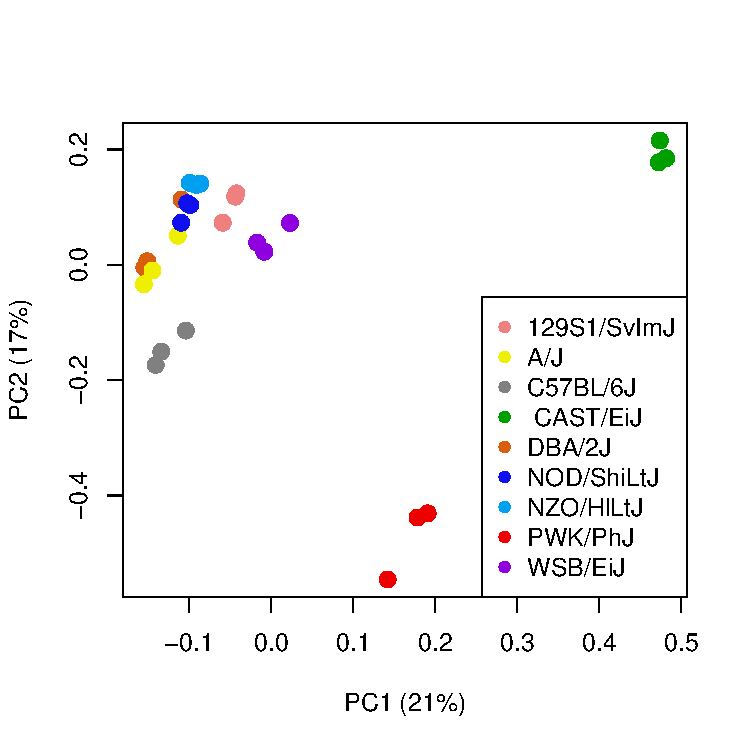
\includegraphics[width=3in]{Figures/Fig1_Decomposition.png} 
\caption{The first two \DIFdelbeginFL \DIFdelFL{principle }\DIFdelendFL \DIFaddbeginFL \DIFaddFL{principal }\DIFaddendFL components of each genomic feature across
nine inbred strains of mouse. In all panels each point represents
an individual mouse, and strain is indicated by color as shown in
the legend at the bottom of the figure. \DIFaddbeginFL \DIFaddFL{Three individuals per strain
are shown. }\DIFaddendFL Each panel is labeled with the data used to generate the 
PC plot. (A) Hepatocyte transcriptome - all transcripts sequenced in 
isolated hepatocytes. (B) DNA methylation - the percent methylation at 
all CpG sites shared across all individuals. (C-F) Histone 
modifications - the peak heights of the indicated histone
modification for sites shared across all individuals.}
\label{fig:pc_plots}
\end{figure}

\hypertarget{chromatin-state-overview}{%
\subsection{Chromatin state overview}\label{chromatin-state-overview}}

\DIFdelbegin \DIFdel{To investigate the association between histone modifications and gene
expression, we }\DIFdelend \DIFaddbegin \DIFadd{We }\DIFaddend used ChromHMM to identify 14 chromatin states composed of unique
combinations of the four histone modifications \DIFdelbegin \DIFdel{. Panel Ain Figure
\ref{fig:state_overview}shows the representation of each histone
modification across the states. }\DIFdelend \DIFaddbegin \DIFadd{(Fig.
\ref{fig:state_overview}A). We calculated the enrichment of each state
near predicted functional elements in the mouse liver (Fig.
\ref{fig:state_overview}B), and correlated the presence of each state
with gene expression both across genes and across the inbred mouse
strains (Fig. \ref{fig:state_overview}C).
}\DIFaddend 

\begin{figure}[ht!]
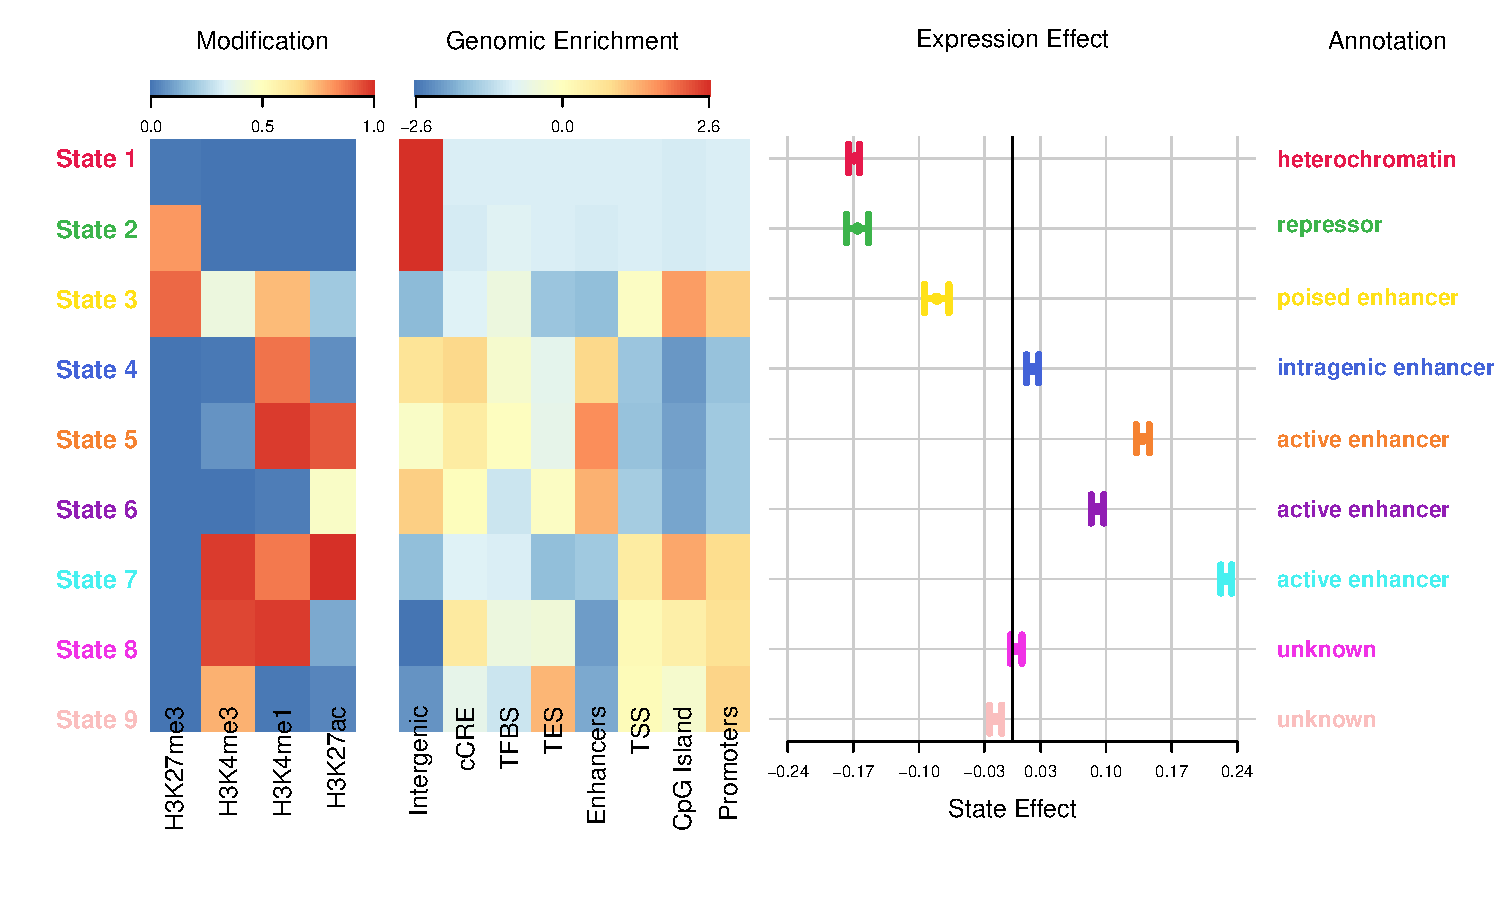
\includegraphics[width=\textwidth]{Figures/Fig2_Overview.png} 
\caption{Overview of chromatin state composition, genomic 
distribution, and effect on expression. (A) Emission 
probabilites for each histone modification in each 
chromatin state. Blue indicates the absence of the histone
modification, and red indicates the presence of the 
modification. (B) The distribution of each state around 
functional elements in the genome. Red indicates that the 
state is enriched near the annotated functional element. 
Blue indicates that the state is depleted near the annotated 
functional element. Abbreviations are as follows: 
\DIFdelbeginFL \DIFdelFL{TFBS }\DIFdelendFL \DIFaddbeginFL \DIFaddFL{Enh. }\DIFaddendFL = \DIFdelbeginFL \DIFdelFL{transcription factor binding sites}\DIFdelendFL \DIFaddbeginFL \DIFaddFL{enhancer}\DIFaddendFL , \DIFdelbeginFL \DIFdelFL{cCRE }\DIFdelendFL \DIFaddbeginFL \DIFaddFL{Tsd }\DIFaddendFL = \DIFdelbeginFL \DIFdelFL{candidate 
cis-regulatory element, TSS = transcription 
}\DIFdelendFL \DIFaddbeginFL \DIFaddFL{distal to the transcript }\DIFaddendFL start site, 
\DIFdelbeginFL \DIFdelFL{TES }\DIFdelendFL \DIFaddbeginFL \DIFaddFL{Tsp }\DIFaddendFL = \DIFaddbeginFL \DIFaddFL{proximal to the }\DIFaddendFL transcription \DIFdelbeginFL \DIFdelFL{end }\DIFdelendFL \DIFaddbeginFL \DIFaddFL{start }\DIFaddendFL site\DIFaddbeginFL \DIFaddFL{; Hetero}\DIFaddendFL . \DIFaddbeginFL \DIFaddFL{= 
heterochromatin; FR = flanking region. }\DIFaddendFL (C) The effect of 
variation in the state on gene expression. Bars are colored 
based on the size and direction the state's effect on expression. 
\DIFdelbeginFL \DIFdelFL{Darker }\DIFdelendFL \DIFaddbeginFL \DIFaddFL{Red/blue }\DIFaddendFL bars show the effects on expression of chromatin state 
variation across strains. \DIFdelbeginFL \DIFdelFL{Tan }\DIFdelendFL \DIFaddbeginFL \DIFaddFL{Blue-gray }\DIFaddendFL bars show the effects on 
expression of chromatin state variation across genes. (D) Plausible 
annotations for each state based on \DIFdelbeginFL \DIFdelFL{combining the data in 
the previous three panels}\DIFdelendFL \DIFaddbeginFL \DIFaddFL{genomic enrichments}\DIFaddendFL . The numbers 
in parentheses indicate the percent of the genome that was assigned 
to each state. \DIFaddbeginFL \DIFaddFL{Repress. = repressor.}\DIFaddendFL }
\label{fig:state_overview}
\end{figure}

\DIFdelbegin \DIFdel{The states were enriched around known functional elements in the mouse
genome (Figure \ref{fig:state_overview}B). For example, the
majority of the states were enriched around transcription
start sites (TSS), and
other TSS-related functional elements, such as promoters and CpG
islands. Two states (States 13 and 14)were primarily found in intergenic regions. Three states (States 2, 6, and 4) were enriched
around known enhancers, and one (State 9) was enriched predominantly
near the transcription end sites (TES).
}\DIFdelend \DIFaddbegin \DIFadd{To associate chromatin state with expression across transcripts, we
calculated the proportion of the gene body that was occupied by each
state in each inbred strain. We then fit a linear model to associate the
proportion of each chromatin state with the amount of transcription
within each strain (Methods). We compared this to the correlation
between chromatin state and gene expression }\emph{\DIFadd{across}} \DIFadd{strains
(Methods). For any given transcript, a strain with more active enhancer
would be expected to have higher expression than a strain with less
active enhancer in that gene. Through this calculation, we can correlate
strain variation in gene expression to strain variation in chromatin
state.
}\DIFaddend 

\DIFdelbegin \DIFdel{Most states were also associated with variation in gene expressionacross strains (Figure \ref{fig:state_overview}C).
The states in Figure \ref{fig:state_overview}are shown in order of their
effect on
expression }\DIFdelend \DIFaddbegin \DIFadd{By merging the histone modification combinations, with functional
element enrichments, and associations with gene expression, we could
assign putative annotatations to each of the 14 chromatin states (Fig.
\ref{fig:state_overview}D).
}

\DIFadd{In Figure \ref{fig:state_overview}, the states are ordered by their
association with gene expression across strains}\DIFaddend , which helps illustrate
several patterns. \DIFaddbegin \DIFadd{Overall, states that were associated with increased
expression across transcripts were also associated with increased
expression when varying across strains. }\DIFaddend The state with the largest
negative \DIFdelbegin \DIFdel{effect on gene expression }\DIFdelend \DIFaddbegin \DIFadd{association with gene expression across strains}\DIFaddend , State 14, \DIFdelbegin \DIFdel{is }\DIFdelend \DIFaddbegin \DIFadd{was
}\DIFaddend the absence of all measured modifications. Other states associated with
reduced gene expression contained the repressive mark H3K27me3. The
states with the largest positive effects on expression all had some
combination of the activating marks, H3K4me3, H3K4me1, and H3K27ac. The
repressive mark was less commonly seen in these activating states.
\DIFdelbegin \DIFdel{These global patterns of positional enrichment and
association with expression largely agree with previous findings}\DIFdelend \DIFaddbegin 

\DIFadd{Except for State 14, all states were enriched around at least one of the
predicted predicted functional elements in mouse liver (Fig.
\ref{fig:state_overview}B). Interestingly, the annotations of these
states largely matched the associations we saw between each state and
gene expression (Fig. \ref{fig:state_overview}C). For example, State 1,
which was enriched around strong enhancers, was the state that was most
strongly corrlated with increased expression both across genes, and
across strains. Likewise, States 2-4 were all enriched around active
enhancers or promoters, and were all correlated with increased
expression overall}\DIFaddend .

\DIFdelbegin \DIFdel{By merging the information from Figure \ref{fig:state_overview}A-C, we
were able to suggest annotations for many of }\DIFdelend \DIFaddbegin \DIFadd{At the other end of the spectrum, state 13 was enriched around polycomb
repressor marks, as we would expect because it was defined by H3K27me3,
which is associated with polycomb repression. This state was also
correlated with reduced expression both across genes and across strains.
}

\DIFadd{Many of the states with weaker effects, both positive and negative were
most enriched around bivalent promoters. This suggests that the bivalent
promoter class may represent a diverse array of functional elements with
varied effects on gene expression, and that more detailed experiments
investigating the relationship between these states and gene expression
could potentially identify novel chromatin states influencing expression
in these cells.
}

\hypertarget{dna-methylation-overview}{%
\subsection{DNA methylation overview}\label{dna-methylation-overview}}

\DIFadd{To investigate the variation in DNA methylation across the the inbred
strains, we examined both strain-specific CpG sites and strain-specific
methylation values. We defined a strain-specific CpG site as one that
was present in all individuals in at least one strain and absent in all
individuals in at least one other strain (Methods).
}

\DIFadd{Across all chromosomes between 16\% and 19\% of CpG sites were
strain-specific (Supplemental Fig. \ref{supp_fig:cpg_overview}A).
Strain-specific CpG sites were more commonly present in CAST, PWK, and
B6 compared to the other strains (Supplemental Fig.
\ref{supp_fig:cpg_overview}B), suggesting that these strains have more
DNA methylation overall compared with the other strains.
}

\DIFadd{CpG sites that were shared across all strain were enriched around
genomic features such as CpG islands and promoters (Methods)
(Supplemental Fig. \ref{supp_fig:cpg_overview}C). Strain-specific CpG
sites were also enriched around CpG sites and promoters (Supplemental
Fig. \ref{supp_fig:cpg_overview}D). However, relative to the CpG sites
found across all strains, }\DIFaddend the \DIFdelbegin \DIFdel{14 chromatin states (Figure \ref{fig:state_overview}D).
States with the strongest effects on
expression had the clearest annotations, while states with weaker
effects remained unannotated.
}\DIFdelend \DIFaddbegin \DIFadd{strain-specific CpG sites were more
strongly enriched specifically in enhancers, especially TSS-distal
poised enhancers and weak enhancers (Supplemental Fig.
\ref{supp_fig:cpg_overview}E). Relative to the CpG sites common across
all strains, strain-specific sites were depleted in promoter regions and
CpG islands (Supplemental Fig. \ref{supp_fig:cpg_overview}E) suggesting
that variation in DNA methylation across strains primarily occurs in
enhancers that fine-tune gene expression levels rather than in promoters
which might result in genes being turned on or off.
}\DIFaddend 

\hypertarget{spatial-distribution-of-epigenetic-modifications-around-gene-bodies}{%
\subsection{Spatial distribution of epigenetic modifications around gene
bodies}\label{spatial-distribution-of-epigenetic-modifications-around-gene-bodies}}

In addition to looking for enrichment of chromatin states \DIFaddbegin \DIFadd{and CpG sites
}\DIFaddend near annotated functional elements, we characterized the fine-grained
spatial distribution of \DIFdelbegin \DIFdel{each state }\DIFdelend \DIFaddbegin \DIFadd{these features }\DIFaddend around gene bodies by normalizing
gene position to run from 0 at the TSS to 1 at the TES (See Methods)
(\DIFdelbegin \DIFdel{Figure
\ref{fig:state_abundance}A-B). We similarly characterized the
distribution of CpG sites and their percent methylation at this
gene-level scale (Figure \ref{fig:state_abundance}C-D)
.
}\DIFdelend \DIFaddbegin \DIFadd{Fig. \ref{fig:state_abundance})
}\DIFaddend 

\begin{figure}[ht!]
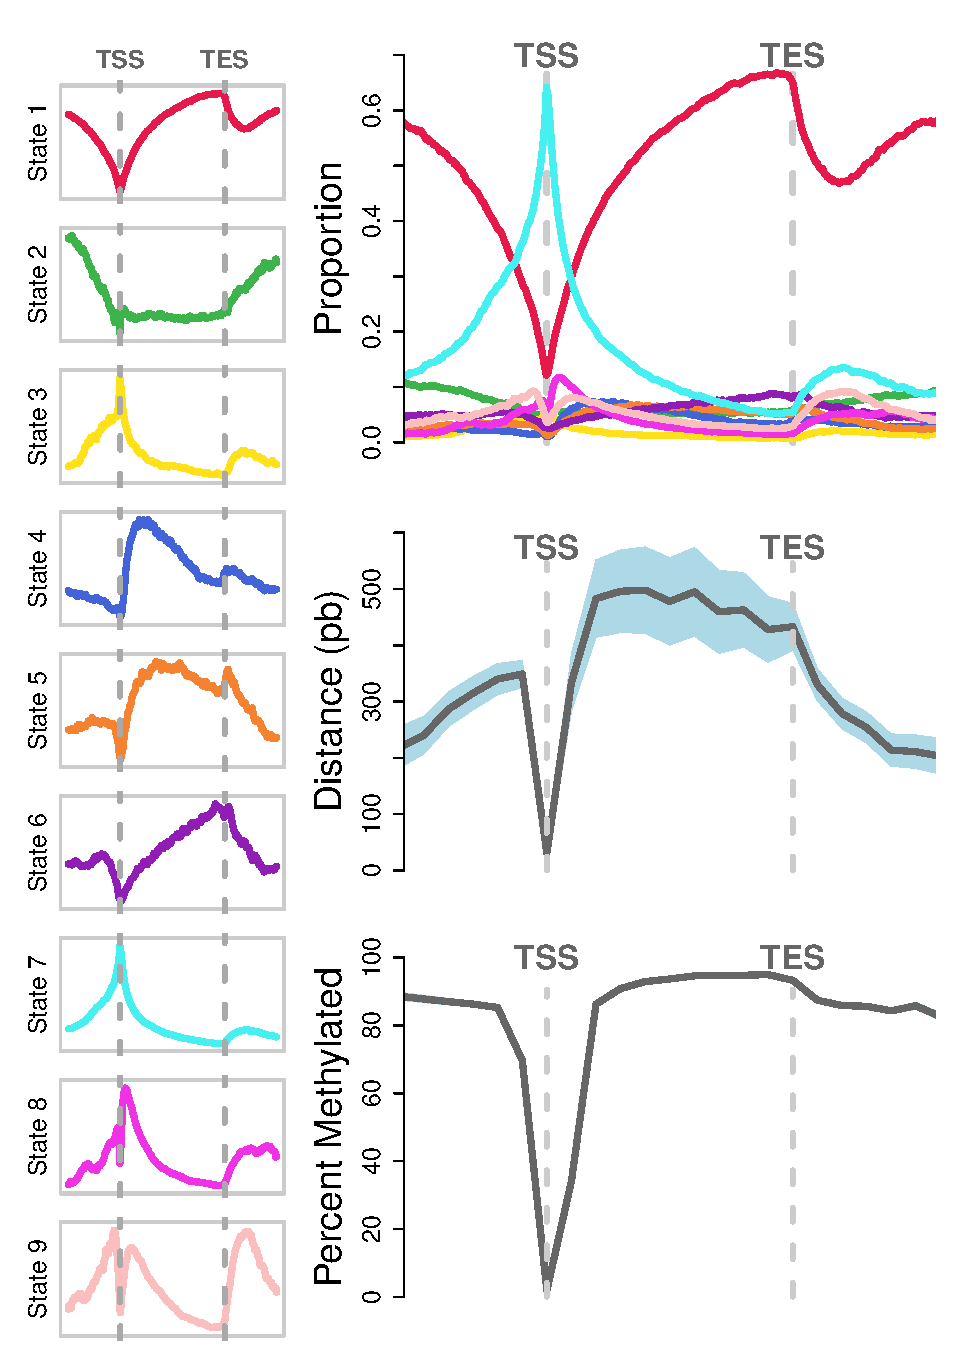
\includegraphics[width=0.67\textwidth]{Figures/Fig3_Abundance.png} 
\caption{Relative abundance of chromatin states and methylated DNA. (A) Each panel 
shows the abundance of a single chromatin state relative to gene TSS and TES. The 
$y$-axis in each panel is the proportion of genes containing the state. Each
panel has an independent $y$-axis to better show the shape of each curve.
The $x$-axis is the relative gene position. The TSS and TES are marked as vertical
gray dashed lines. (B) The same data shown in panel A, but with all states overlayed
onto a single set of axes to show the relative abundance of the states. 
(C) The density of CpG sites relative to the gene body. The $y$-axis shows the 
number of CpG sites per base pair. The density is highest near the TSS. 
CpG sites are less dense within the gene body and in the intergenic space. 
(D) Percent methylation relative to the gene body. The $y$-axis shows the median 
percent methylation at CpG sites, and the $x$-axis shows relative gene position. 
CpG sites near the TSS are unmethylated relative to intragenic \DIFaddbeginFL \DIFaddFL{sites }\DIFaddendFL and \DIFdelbeginFL \DIFdelFL{intergenic
CpG }\DIFdelendFL \DIFaddbeginFL \DIFaddFL{to }\DIFaddendFL sites
\DIFaddbeginFL \DIFaddFL{just upstream and downstream of the gene bodies}\DIFaddendFL . \DIFaddbeginFL \DIFaddFL{In both C and D standard error 
is shown as a blue envelope around the mean; however, the standard error is so 
small that it is not visible in the figure.}\DIFaddendFL }
\label{fig:state_abundance}
\end{figure}

The spatial patterns of the individual chromatin states are shown in
(\DIFdelbegin \DIFdel{Figure }\DIFdelend \DIFaddbegin \DIFadd{Fig. }\DIFaddend \ref{fig:state_abundance}A), and an overlay of all states together
(\DIFdelbegin \DIFdel{Figure }\DIFdelend \DIFaddbegin \DIFadd{Fig. }\DIFaddend \ref{fig:state_abundance}B) emphasizes the difference in abundance
between the most abundant states (States 1, 3, and 14), and the
remaining states, which were relatively rare.

Each chromatin state had a characteristic distribution pattern \DIFaddbegin \DIFadd{across
the gene body}\DIFaddend . For example, State 14, which was characterized by the
absence of all measured histone modifications, was strongly depleted
near the TSS, indicating that this region is commonly subject to the
histone modifications we measured here. \DIFaddbegin \DIFadd{It should be noted this this
pattern is independent of the global enrichment patterns shown in Figure
\ref{fig:state_overview}. Although state 14 is generally depleted in
gene bodies relative to intergenic regions, it is especially depleted at
the TSS. }\DIFaddend In contrast, States 1 and 3 were both \DIFdelbegin \DIFdel{enriched }\DIFdelend \DIFaddbegin \DIFadd{relatively abundant }\DIFaddend at
the TSS. State 3 was very narrowly concentrated right at the TSS,
\DIFdelbegin \DIFdel{whereas }\DIFdelend \DIFaddbegin \DIFadd{consistent with its annotation as an active promoter (Fig.
\ref{fig:state_overview}). }\DIFaddend State 1 \DIFdelbegin \DIFdel{was more broadly abundant both upstream and
downstream }\DIFdelend \DIFaddbegin \DIFadd{on the other hand, was especially
enriched just upstream }\DIFaddend of the TSS\DIFdelbegin \DIFdel{. Both were associated overall with increased
expression across inbred mice (indicated by red shading in Figure
\ref{fig:state_abundance}), suggesting promoter or enhancerfunctions. The third state in this group of expression-enhancing states, }\DIFdelend \DIFaddbegin \DIFadd{, consistent with its annotation of a
TSS-proximal strong enhancer. }\DIFaddend State 2, was depleted nere the TSS, but
enriched within the gene body, \DIFdelbegin \DIFdel{suggesting
that this state may mark active intragenic enhancers}\DIFdelend \DIFaddbegin \DIFadd{consistent with its annotation of a
TSS-distal enhancer}\DIFaddend .

States with weaker \DIFdelbegin \DIFdel{effects on }\DIFdelend \DIFaddbegin \DIFadd{associations to }\DIFaddend expression (indicated by grayer
shades in \DIFdelbegin \DIFdel{Figure }\DIFdelend \DIFaddbegin \DIFadd{Fig. }\DIFaddend \ref{fig:state_abundance}) were of lower abundance, but
had distinct distribution patterns around the gene body suggesting the
possibility of distinct functional roles in the regulation of gene
expression. \DIFaddbegin \DIFadd{The abundance patterns were identical across all strains
(Supplemental Fig. \ref{supp_fig:state_abundance_by_strain})
}\DIFaddend 

DNA methylation showed similarly characteristic variation in abundance
(\DIFdelbegin \DIFdel{Figure }\DIFdelend \DIFaddbegin \DIFadd{Fig. }\DIFaddend \ref{fig:state_abundance}C-D). The TSS had densely packed CpG
sites relative to the gene body (\DIFdelbegin \DIFdel{Figure }\DIFdelend \DIFaddbegin \DIFadd{Fig. }\DIFaddend \ref{fig:state_abundance}C). As
expected, the median CpG site near the TSS was consistently
hypomethylated relative to the median CpG site in intra- and intergenic
regions (\DIFdelbegin \DIFdel{Figure }\DIFdelend \DIFaddbegin \DIFadd{Fig. }\DIFaddend \ref{fig:state_abundance}D). All genes used in this
analysis were expressed and thus had some degree of hypomethylation.
\DIFaddbegin \DIFadd{There were also no large-scale difference in CpG distribution or percent
methylation across strains (Supplemental Fig.
\ref{supp_fig:percent_methyl_by_strain}).
}\DIFaddend 

\hypertarget{spatially-resolved-effects-on-gene-expression}{%
\subsection{Spatially resolved effects on gene
expression}\label{spatially-resolved-effects-on-gene-expression}}

The distinct spatial distributions of the chromatin states and
methylated CpG sites around the gene body raised the question as to
whether the effects of these states on gene expression could also be
spatially resolved. To investigate this possibility we tested the
association between gene expression and both chromatin state and DNA
methylation using spatially resolved models (Methods). We tested the
effect of each chromatin state on expression across genes within
hepatocytes (\DIFdelbegin \DIFdel{Figure }\DIFdelend \DIFaddbegin \DIFadd{Fig. }\DIFaddend \ref{fig:state_effects}A) and the effect of each
chromatin state on the variation in gene expression across strains (\DIFdelbegin \DIFdel{Figure }\DIFdelend \DIFaddbegin \DIFadd{Fig.
}\DIFaddend \ref{fig:state_effects}B).

\begin{figure}[ht!]
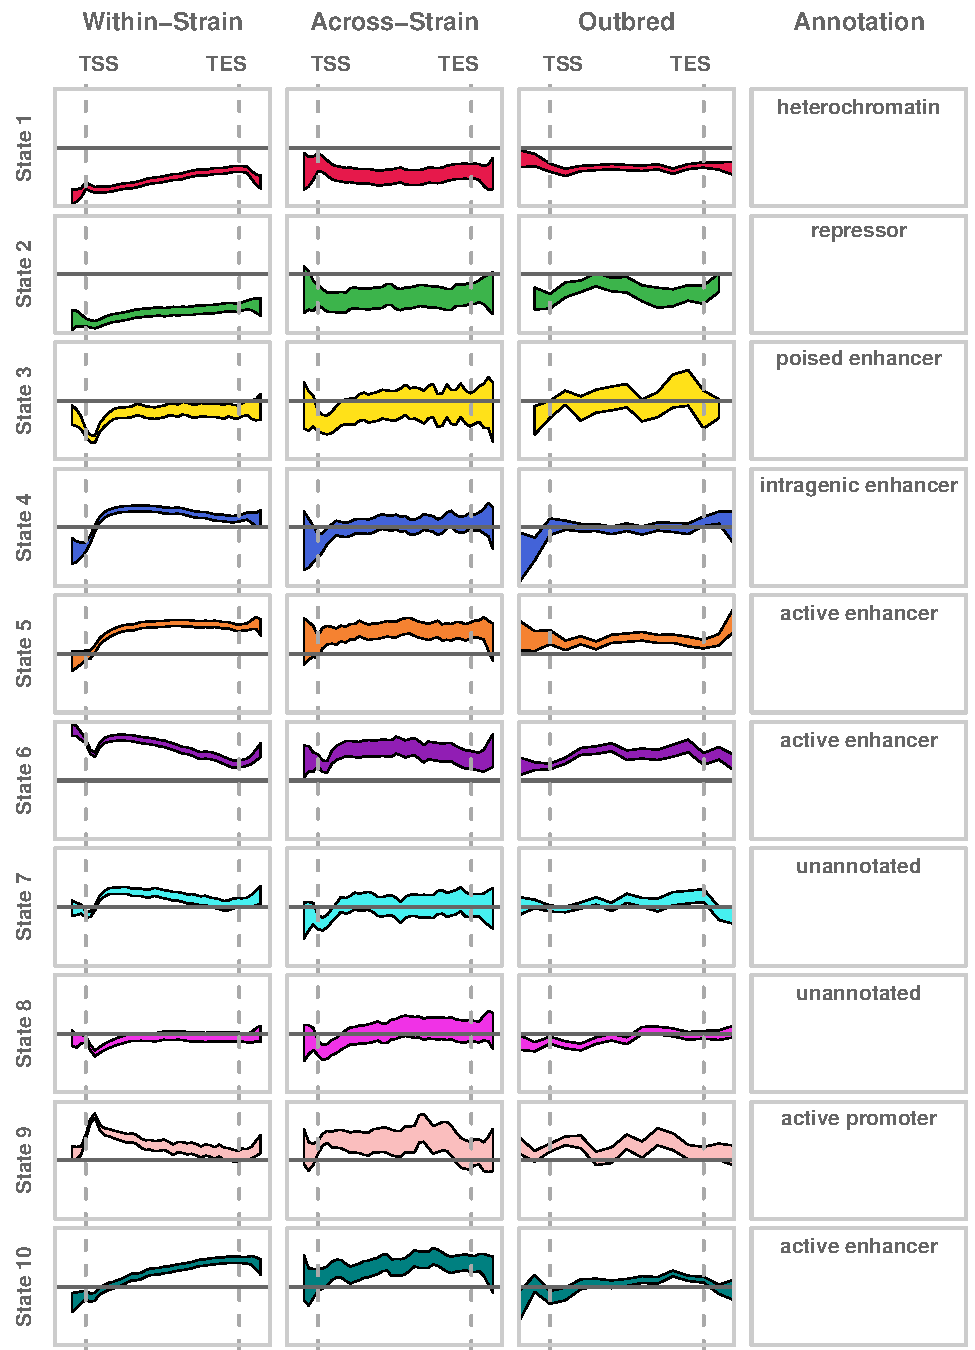
\includegraphics[width=0.7\textwidth]{Figures/Fig4_Effects.png}
\caption{Effects of chromatin states on gene expression. Each column shows 
the effect of \DIFdelbeginFL \DIFdelFL{the }\DIFdelendFL \DIFaddbeginFL \DIFaddFL{each }\DIFaddendFL chromatin \DIFdelbeginFL \DIFdelFL{states }\DIFdelendFL \DIFaddbeginFL \DIFaddFL{state }\DIFaddendFL on gene expression in a different 
experimental context. The first column shows \DIFdelbeginFL \DIFdelFL{that }\DIFdelendFL the \DIFdelbeginFL \DIFdelFL{presence }\DIFdelendFL \DIFaddbeginFL \DIFaddFL{effect across genes in 
the inbred mice showing how chromatin states are used within hepatocytes 
to increase the expression }\DIFaddendFL of some \DIFdelbeginFL \DIFdelFL{states is correlated with higher abundance }\DIFdelendFL genes \DIFdelbeginFL \DIFdelFL{while }\DIFdelendFL \DIFaddbeginFL \DIFaddFL{and decrease }\DIFaddendFL the \DIFdelbeginFL \DIFdelFL{presence }\DIFdelendFL \DIFaddbeginFL \DIFaddFL{expression 
}\DIFaddendFL of other \DIFdelbeginFL \DIFdelFL{states is correlated with lower abundance }\DIFdelendFL genes\DIFdelbeginFL \DIFdelFL{in mouse hepatocytes}\DIFdelendFL . The second column shows \DIFdelbeginFL \DIFdelFL{that variation in }\DIFdelendFL \DIFaddbeginFL \DIFaddFL{the effect of }\DIFaddendFL chromatin state 
\DIFdelbeginFL \DIFdelFL{across strains
is correlated with variation in }\DIFdelendFL \DIFaddbeginFL \DIFaddFL{on }\DIFaddendFL gene expression \DIFaddbeginFL \DIFaddFL{across strains}\DIFaddendFL . The third column shows the effect 
of imputed chromatin state on gene expression in a population of \DIFdelbeginFL \DIFdelFL{DO }\DIFdelendFL \DIFaddbeginFL \DIFaddFL{diversity 
outbred }\DIFaddendFL mice. \DIFdelbeginFL \DIFdelFL{The $y$-axis }\DIFdelendFL \DIFaddbeginFL \DIFaddFL{These plots show the effect on local gene expression of 
variation }\DIFaddendFL in \DIFdelbeginFL \DIFdelFL{each }\DIFdelendFL \DIFaddbeginFL \DIFaddFL{chromatin state across genetically diverse individuals. 
Each }\DIFaddendFL column \DIFaddbeginFL \DIFaddFL{of panels }\DIFaddendFL is \DIFdelbeginFL \DIFdelFL{constant }\DIFdelendFL \DIFaddbeginFL \DIFaddFL{plotted on a single scale }\DIFaddendFL for \DIFdelbeginFL \DIFdelFL{comparison
}\DIFdelendFL \DIFaddbeginFL \DIFaddFL{the $y$-axis so 
the magnitude }\DIFaddendFL of \DIFdelbeginFL \DIFdelFL{states }\DIFdelendFL \DIFaddbeginFL \DIFaddFL{the effects in a single column can be compared directly 
}\DIFaddendFL to each other\DIFdelbeginFL \DIFdelFL{within a single context}\DIFdelendFL . \DIFdelbeginFL \DIFdelFL{The }\DIFdelendFL \DIFaddbeginFL \DIFaddFL{All }\DIFaddendFL $y$-axes \DIFdelbeginFL \DIFdelFL{vary across
columns }\DIFdelendFL \DIFaddbeginFL \DIFaddFL{are centered around 0 (black horizontal line). 
Across a single row, the scale of the $y$-axis varies }\DIFaddendFL to highlight the 
similarity of the shape of each curve \DIFdelbeginFL \DIFdelFL{across 
settings}\DIFdelendFL \DIFaddbeginFL \DIFaddFL{in each different setting}\DIFaddendFL . \DIFaddbeginFL \DIFaddFL{Values 
above the zero line indicate a positive correlation between the state and 
gene expression at that genomic position. Labels on the $y$-axis in the 
first column are in arbitrary units and indicate where the 0 line is as 
well as positive and negative effects. Values below the zero line indicate 
a negative correlation between the state and gene expression at that genomic 
positin. }\DIFaddendFL The \DIFaddbeginFL \DIFaddFL{colored areas indicate the 95\% confidence interval around the 
mean estimate. The }\DIFaddendFL final column shows the annotation of each state \DIFaddbeginFL \DIFaddFL{for 
comparison with its effects on gene expression}\DIFaddendFL . All $y$-axes show the 
$\beta$ coefficient from the linear model shown in \DIFdelbeginFL \DIFdelFL{the }\DIFdelendFL equation \DIFdelbeginFL \DIFdelFL{. 
}\DIFdelendFL \DIFaddbeginFL \DIFaddFL{1. }\DIFaddendFL All 
$x$-axes show the relative position along the gene body \DIFaddbeginFL \DIFaddFL{running from 
just upstream of the TSS to just downstream of the TES}\DIFaddendFL . Vertical gray 
dashed lines mark the TSS and TES \DIFaddbeginFL \DIFaddFL{in all panels}\DIFaddendFL .
}
\label{fig:state_effects}
\end{figure}

All chromatin states demonstrated spatially dependent effects on gene
expression within hepatocytes. \DIFaddbegin \DIFadd{Figure \ref{fig:state_effects} shows how
these effects are distributed across the states and across the gene
bodies. In each panel the \(y\)-axis is centered around zero (black
horizontal line). Effects above this line indicate the state had a
positive association with gene expression, whereas effects below the
center line show the state had a negative correlation with gene
expression at that particular position.
}

\DIFaddend For many of the states, the effects on expression were concentrated at
or near the TSS, while in the other states effects were seen across the
whole gene. The direction of the effects matched the overall effects of
each state seen previously (\DIFdelbegin \DIFdel{Figure \ref{fig:state_overview}). The spatial effects were
recapitulated for almost every state when we measured across strains .
}\DIFdelend \DIFaddbegin \DIFadd{Fig. \ref{fig:state_overview}), but here we
see finer resolution on the effect. For example, State 3 was positively
correlated overall with gene expression (Fig.
\ref{fig:state_overview}C), but in Figure \ref{fig:state_effects} we see
that this positive correlation is primarily limited to the region near
the TSS, consistent with its annotation as a promoter state.
}

\DIFadd{Further, the spatial effects observed across genes (Fig.
\ref{fig:state_effects} first column) were largely recapitulated in the
measurements across strains (Fig. \ref{fig:state_effects} middle
column). }\DIFaddend That is, chromatin states that either enhanced or suppressed
gene expression across hepatocyte genes were similarly related to
variation in expression across strains. This suggests that the genetic
differences between strains modify chromatin activity in a manner
similar to that used across genes. One notable exception was State 6,
whose presence upregulated genes within hepatocytes, but did not
contribute to expression variation across strains.

We also examined the effect of percent DNA methylation across genes
within hepatocytes and across strains (\DIFdelbegin \DIFdel{Figure
}\DIFdelend \DIFaddbegin \DIFadd{Fig.
}\DIFaddend \ref{fig:DNA_methylation_effect}). As expected, methylation at the TSS
was associated with lower \DIFdelbegin \DIFdel{expression in hepatocytes . However, percent
DNA methylation did not contribute at all to expression variation across strains. This was in part due to an overall lack of variation in percent
DNA methylation
at the TSS.
These results imply that percent DNA methylation does not vary significantly between strains, at least in
hepatocytes, and does not contribute to variation in gene expression
across }\DIFdelend \DIFaddbegin \DIFadd{expressed genes in hepatocytes (Fig.
\ref{fig:DNA_methylation_effect}A). We did not detect an association
between DNA methylation percent and gene expression across inbred
strains, perhaps because there were too few strains to reliabley
estimate the effects (Fig. \ref{fig:DNA_methylation_effect}B). However,
we did see a significant negative association between DNA methylation
and gene expression when we imputed DNA methylation in the DO (Fig.
\ref{fig:DNA_methylation_effect}C). These results suggest that heritably
DNA methylation contributes significantly to eQTL in }\DIFaddend genetically diverse
individuals.

\begin{figure}[ht!]
\includegraphics[width=3in]{Figures/Fig5_methylation_effect.png} 
\caption{Effect of DNA methylation on gene expression (A) across gene expression
in hepatocytes and (B) across inbred strains. The dark gray line shows the
estimate of the effect of percent DNA methylation on gene expression. The 
$x$-axis is normalized position along the gene body running from the 
transcription start site (TSS) to the transcription end site (TES), 
marked with vertical gray dashed lines. The horizontal solid black 
line indicates an effect of 0. The shaded gray area shows 95\% 
confidence interval arond the model fit.}
\label{fig:DNA_methylation_effect}
\end{figure}

\DIFdelbegin %DIFDELCMD < \hypertarget{imputed-chromatin-state-explained-expression-variation-in-diversity-outbred-mice}{%
%DIFDELCMD < \subsection{Imputed chromatin state explained expression variation in
%DIFDELCMD < diversity outbred
%DIFDELCMD < mice}\label{imputed-chromatin-state-explained-expression-variation-in-diversity-outbred-mice}}
%DIFDELCMD < %%%
\DIFdelend \DIFaddbegin \hypertarget{interactions-between-chromatin-state-and-dna-methylation}{%
\subsection{Interactions between chromatin state and DNA
methylation}\label{interactions-between-chromatin-state-and-dna-methylation}}
\DIFaddend 

\DIFdelbegin \DIFdel{Thus far, we have used inbred strains of miceto identify correlations
between local chromatin state and gene expression. To compare the contribution of genetic and epigenetic features to expression quantitative trait loci (eQTLs)in a gentically diverse population, we
imputed chromatin state
}\DIFdelend \DIFaddbegin \DIFadd{We investigated whether there was an interaction between DNA methylation
and chromatin state by asking two questions. First, were CpG sites
within different chromatin states methylated at different levels? And
second, was DNA methylation within specific chromatin states
differentially associated with gene expression across inbred mice? If
DNA methylation essentially inactivates a region of DNA, methylation in
a region identified as a repressor based on its chromatin state might be
expected to increase gene expression, whereas methylation in an active
enhancer might decrease gene expression.
}

\DIFadd{To investigate these questions, we identified CpG sites within each of
the 14 chromatin states. We calculated the average percent methylation
of these sites, and the effect of DNA methylation on gene expression for
each set of sites (Methods). We treated missing CpG sites in individual
strains as unmethylated.
}

\DIFadd{Although methylation patterns in all states followed roughly the same
pattern of unmethylated at the transcription start site and methylated
within the gene body, values ranged widely across the states from State
3 with a mean of 27\% methylated DNA intragenically, to State 14 with
83\% methylated DNA intragenically. Again, these differential levels of
methylation within these states are consistent with the state
annotations. State 3 was annotated as an active promoter, and we would
expect DNA methylation in this state to be low. State 14 has no histone
modifications and is not expected to be transcriptionally active, which
is consistent with high levels of DNA methylation.
}

\DIFadd{DNA methylation in a subset of the chromatin states was significantly
correlated with gene expression (Supplemental Fig.
\ref{supp_fig:methyl_effect_by_state}). DNA methylation in State 3, the
active promoter state}\DIFaddend , \DIFdelbegin \DIFdel{DNA methylation, and SNPs into DO mice
(Methods). Chromatin stateis largely determined by local genotype, especially early in life \mbox{%DIFAUXCMD
\citep{pmid16009939}}\hspace{0pt}%DIFAUXCMD
,
and can thus be reliably
imputed from local genotype. Further, we have shown here that local
chromatin state correlates with variation in gene expressionacross
inbred strains. DNA methylation, on the other hand, is known not to be highly heritable \mbox{%DIFAUXCMD
\citep{pmid33931130}}\hspace{0pt}%DIFAUXCMD
, and thus cannot be reliably
imputed from local genotype. We have also shown here that DNA methylation is not correlated with variation in }\DIFdelend \DIFaddbegin \DIFadd{was associated with decreased gene expression,
suggesting that DNA methylation in this state deactivated the active
promoter state. Overall, State 11, a state annotated as a bivalent
promoter, was negatively associated with }\DIFaddend gene expression\DIFdelbegin \DIFdel{across
inbred strains. The imputation of DNA methylation thus serves as a
negative control--an estimate of a lower bound the ability of a feature
imputed from local haplotype to
explain gene expression in a new
population}\DIFdelend . \DIFaddbegin \DIFadd{However, DNA
methylation in this state was positively associated with gene
expression, suggesting that this repressive state can be inactivated by
DNA methylation.
}\DIFaddend 

\DIFdelbegin \DIFdel{After imputing each genomic feature }\DIFdelend \DIFaddbegin \hypertarget{imputed-chromatin-state-explained-expression-variation-in-diversity-outbred-mice}{%
\subsection{Imputed chromatin state explained expression variation in
diversity outbred
mice}\label{imputed-chromatin-state-explained-expression-variation-in-diversity-outbred-mice}}

\DIFadd{Thus far, we have shown correlations between gene expression and
epigenetic features in inbred mice. We were also interested in whether
chromatin state and DNA methylation were associated with gene expression
in an outbred mouse population. Although we did not measure epigenetic
modifications directly in an outbred population, we had liver gene
expression from a previously published population of diversity outbred
mice \mbox{%DIFAUXCMD
\citep{pmid28592500}}\hspace{0pt}%DIFAUXCMD
. Inheritance of chromatin state and DNA
methylation is complex \mbox{%DIFAUXCMD
\citep{rintisch2014natural}}\hspace{0pt}%DIFAUXCMD
; however there is
evidence that the heritability for both epigenetic features is high
\mbox{%DIFAUXCMD
\citep{pmid16009939,pmid33931130} }\hspace{0pt}%DIFAUXCMD
suggesting the possibility of imputing
epigenetic features from local genotype into the DO mice. Even with
imperfect estimates of epigenetic features in the outbred mice, a common
pattern of association between outbred and inbred mice would support the
idea that inherited variance in epigenetic features contributes to
inherited variation in gene expression across genetically distinct
individuals.
}

\DIFadd{We imputed chromatin state, DNA methylation, and SNPs }\DIFaddend into the DO
population \DIFdelbegin \DIFdel{, we mapped
gene expressionto the imputed features and calculated the variance
explained }\DIFdelend \DIFaddbegin \DIFadd{(Methods). Because any feature imputed from haplotype will be
correlated with gene expression, we performed permutations that shuffled
the relationship between haplotype and chromatin state }\DIFaddend (Methods). The
\DIFdelbegin \DIFdel{overall distributions of variance explained by
each feature across all transcripts are shown in Figure
\ref{fig:effect_distrubutions}}\DIFdelend \DIFaddbegin \DIFadd{resulting \(p\)-value distributions of each genomic feature suggested
that each imputed feature was significantly associated with gene
expression in the DO beyond the effects of the imputation alone}\DIFaddend .

\DIFdelbegin %DIFDELCMD < \begin{figure}[ht!]
%DIFDELCMD < \includegraphics[width=\textwidth]{Figures/Fig6_Imputation.png} 
%DIFDELCMD < %%%
%DIFDELCMD < \caption{%
{%DIFAUXCMD
\DIFdelFL{Gene expression variance in a DO population explained 
by chromatin state compared to three other genomic features: 
local haplotype, local SNP genotype, and local imputed DNA 
methylation status. A. Distributions of gene expression variance 
explained by each feature. B. Direct comparisons of 
variance explained by local haplotype, and each of the other 
genomic features. Blue lines show $y = x$. Each point is a 
single transcript.}}
%DIFAUXCMD
%DIFDELCMD < \label{fig:effect_distrubutions}
%DIFDELCMD < \end{figure}
%DIFDELCMD < 

%DIFDELCMD < %%%
\DIFdel{These distributions show the haplotype effect for the marker nearest
each transcript compared with the maximum effect across the gene body
for each of the other imputed features. Overall, local haplotype
explained the largest amount of variance of }\DIFdelend \DIFaddbegin \DIFadd{We then tested the association between each chromatin state, each SNP,
or each CpG site with gene expression in the DO. We tested each state
independently to constrain the degrees of freedom for each feature to
one. In parallel, we tested the association between each local haplotype
state and }\DIFaddend gene expression in the DO\DIFdelbegin \DIFdel{(\(R^2 = 0.17\); 99\% CI = 0.166-0.174). The variance explained by local
chromatin statewas very highly correlated with that of haplotype
(Pearson \(r = 0.96\), 99\% CI = 0.958-0.962) and explained almost as
much }\DIFdelend \DIFaddbegin \DIFadd{. This is not the standard method for
testing associations between markers and gene expression in this type of
population, but it constrains the degrees of freedom to one so we can
compare the effect of each individual haplotype to each individual
chromatin state.
}

\DIFadd{Haplotypes are a measure of ancestry, whereas chromatin state, DNA
methylation, and SNPs are all potentially functional variation in the
genome. Thus any individual chromatin state, SNP, or CpG site can
theoretically explain more }\DIFaddend variance in gene expression \DIFdelbegin \DIFdel{in the DO as local haplotype(\(R^2 = 0.15\), 99\% CI = 0.143-0.151).
The mean }\DIFdelend \DIFaddbegin \DIFadd{than an
individual haplotype.
}

\DIFadd{Figure \ref{fig:effect_distrubutions} compares the }\DIFaddend variance explained by
\DIFdelbegin \DIFdel{SNPs was lower (\(R^2 = 0.13\); 99\% CI = 0.131-0.138) than }\DIFdelend \DIFaddbegin \DIFadd{individual haplotypes with }\DIFaddend that explained by \DIFdelbegin \DIFdel{haplotype and was not as highly correlated with local
haplotype as chromatin
statewas (Pearson \(r = 0.93\); 99\%CI =
0.927-0.933). DNA methylation , the lower bound for }\DIFdelend \DIFaddbegin \DIFadd{any individual chromatin
state, CpG site, or SNP. All imputed features--individual chromatin
states (14\%), DNA methylation (14\%), and SNPs (13\%)--explained more
variance than individual haplotypes (11\%) (Fig.
\ref{fig:effect_distrubutions}A). This suggests that any given chromatin
state, CpG site, or SNP carries more functional inforation than an
individual haplotype, which is primarily a measurement of ancestry.
}

\DIFadd{Figure \ref{fig:effect_distrubutions}B shows the maximum }\DIFaddend variance
explained by \DIFdelbegin \DIFdel{a feature imputed from local haplotype, explained the lowest amount of expression variance in the DO population (\(R^2 = 0.09\); 99\% CI =
0.082-0.088), and had a much lower correlation to haplotype than either
chromatin state or SNPs (Pearson \(r = 0.74\); 99\% CI = 0.728-0.751).
Taken together, these results suggest that the }\DIFdelend \DIFaddbegin \DIFadd{each genomic feature for each transcript in the
transcriptome. Dots above the line indicate transcripts for which the
imputed genomic feature explained more variance than haplotype. Dots
below the line indicate transcripts for which the imputed genomic
feature explained less variance than haplotype. Individual haplotype
explained less variance than any other genomic feature for the }\DIFaddend majority
of \DIFdelbegin \DIFdel{haplotype-associated variance is encoded by the chromatin state of the
allele
}\DIFdelend \DIFaddbegin \DIFadd{transcripts. supporting the hypothesis that all these features cary
heritable information that potentially regulates gene expression in this
genetically diverse population.
}

\begin{figure}[ht!]
\includegraphics[width=\textwidth]{Figures/Fig6_Imputation.png} 
\caption{\DIFaddFL{Gene expression variance in a DO population explained 
by chromatin state compared to three other genomic features: 
local haplotype, local SNP genotype, and local imputed DNA 
methylation status. A. Distributions of gene expression variance 
explained by each feature. B. Direct comparisons of 
variance explained by local haplotype, and each of the other 
genomic features. Blue lines show $y = x$. Each point is a 
single transcript.}}
\label{fig:effect_distrubutions}
\end{figure}

\DIFadd{For any gene whose variance was explained at least as well by an imputed
feature as by haplotype, there is the possibility that the imputed
feature marks a cis-regulatory element. This occurence provides an
opportunity to annotate novel functional elements in the mouse genome,
or provide supportive evidence of previously predicted functional
elements. As an example, we investigated the gene }\textit{\DIFadd{Pkd2}} \DIFadd{(Fig.
\ref{fig:example_gene})}\DIFaddend .
\DIFdelbegin \DIFdel{Moreover, this encoding is primarily local and present in the
relevant inbred founder strain.
}\DIFdelend 

\DIFaddbegin \DIFadd{For }\textit{\DIFadd{Pkd2}}\DIFadd{, WSB and PWK were low-expressing strains, and the
remaining strains had higher expression (Fig. \ref{fig:example_gene}E).
The haplotype effects in the DO mirror this pattern with the CAST allele
showing an especially high association with increased gene expression.
}

\DIFaddend To investigate whether natural variation in chromatin state can be used
to \DIFdelbegin \DIFdel{functionally annotate }\DIFdelend \DIFaddbegin \DIFadd{identify putative }\textit{\DIFadd{cis}} \DIFadd{regulatory regions }\DIFaddend the mouse genome,
we looked at the relationship between chromatin state and gene
expression in individual genes. An example gene, \textit{Pkd2}, is shown
in Figure \ref{fig:example_gene}. This figure shows chromatin state
(\DIFdelbegin \DIFdel{Figure }\DIFdelend \DIFaddbegin \DIFadd{Fig. }\DIFaddend \ref{fig:example_gene}B), SNP genotype (\DIFdelbegin \DIFdel{Figure }\DIFdelend \DIFaddbegin \DIFadd{Fig.
}\DIFaddend \ref{fig:example_gene}C), and DNA methylation (\DIFdelbegin \DIFdel{Figure
}\DIFdelend \DIFaddbegin \DIFadd{Fig.
}\DIFaddend \ref{fig:example_gene}D) status along the gene body of \textit{Pkd2}. It
also shows the association of each of these features with gene
expression calculated across the whole gene body (\DIFdelbegin \DIFdel{Figure
}\DIFdelend \DIFaddbegin \DIFadd{Fig.
}\DIFaddend \ref{fig:example_gene}A).

The detailed view of this gene identifies two particularly interesting
regions \DIFdelbegin \DIFdel{. }\DIFdelend \DIFaddbegin \DIFadd{(gray arrows Fig. \ref{fig:example_gene}A). }\DIFaddend One is at the TSS
and the immediately surrounding area, and the other is just downstream
of the TSS.

\begin{figure}[ht!]
\includegraphics[width=0.8\textwidth]{Figures/Fig7_Example.png} 
\caption{Example of epigenetic states and \DIFdelbeginFL \DIFdelFL{imuptation }\DIFdelendFL \DIFaddbeginFL \DIFaddFL{imputation }\DIFaddendFL results for a single 
gene, \textit{Pkd2}. The legend for each panel is displayed to its right.
(A) The variance in DO gene expression explained at 
each position along the gene body by each of the imputed genomic 
features: SNPs - red X's, Chromatin State - blue plus signs, and 
Percent Methylation - green circles. The horizontal 
dashed line shows the \DIFaddbeginFL \DIFaddFL{maximum }\DIFaddendFL variance explained by \DIFdelbeginFL \DIFdelFL{the }\DIFdelendFL \DIFaddbeginFL \DIFaddFL{any individual 
}\DIFaddendFL haplotype \DIFaddbeginFL \DIFaddFL{(in this case CAST)}\DIFaddendFL . For reference, the arrow below 
this panel runs from the TSS of \textit{Pkd2} \DIFaddbeginFL \DIFaddFL{(vertical bar) }\DIFaddendFL to the 
TES \DIFaddbeginFL \DIFaddFL{(arrow head) }\DIFaddendFL and shows the direction of transcription. \DIFaddbeginFL \DIFaddFL{The 
gray arrows at the top indicate two regions of interest where 
chromatin state explains height amounts of variance in gene expression. 
}\DIFaddendFL (B) The chromatin states assigned to each 200 bp window in this gene 
for each inbred mouse strain. States are colored by their effect on 
gene expression in the inbred mice. Red indicates a positive effect 
on gene expression, and blue indicates a negative effect. Each row 
shows the chromatin states for a single inbred strain, which is 
indicated by the label on the left. (C) SNPs along the gene body for 
each inbred strain. The reference genotype is shown in gray. SNPs are 
colored by genotype as shown in the legend. (D) Percent DNA methylation 
for each inbred strain along the \textit{Pkd2} gene body. Percentages 
are binned into 0\% (blue) 50\% (yellow) and 100\% (red). (E) Haplotype 
effects for expression of \textit{Pkd2} in the DO. Haplotype effects 
are colored by from which each allele was derived. (F) \textit{Pkd2} 
expression levels across inbred mouse strains. For ease of comparison, 
all panels B through F are shown in the same order as the haplotype effects.}
\label{fig:example_gene}
\end{figure}

These two regions were both strongly associated expression levels (\DIFdelbegin \DIFdel{Figure }\DIFdelend \DIFaddbegin \DIFadd{Fig.
}\DIFaddend \ref{fig:example_gene}A). Those strains with activating histone states
in these regions had much higher expression of \textit{Pkd2} than the
two strains that did not have activating states in this region. We
hypothesize that these two regions are enhancers.

The spatial patterns in the SNPs only partially mirror those in
chromatin state (\DIFdelbegin \DIFdel{Figure Figure }\DIFdelend \DIFaddbegin \DIFadd{Fig. }\DIFaddend \ref{fig:example_gene}C). SNPs underlying the
putative enhancer region at the TSS could potentially influence gene
expression by altering local chromatin state. However, the more
downstream enhancer has no underlying SNPs, suggesting that there is an
alternative mechanism for determining chromatin state at this location.
Perhaps SNPs in the TSS region regulate both enhancers.

Percent DNA methylation does not vary across the strains in either of
these putative enhancer regions, and does not contribute to variation in
expression across genetically distinct individuals (\DIFdelbegin \DIFdel{Figure
}\DIFdelend \DIFaddbegin \DIFadd{Fig.
}\DIFaddend \ref{fig:example_gene}D).

\hypertarget{discussion}{%
\section{Discussion}\label{discussion}}

In this study we showed that genetic variation across inbred mice \DIFdelbegin \DIFdel{alters
histone modification patterns }\DIFdelend \DIFaddbegin \DIFadd{is
associated with variation in histone modifications and DNA methylation
}\DIFaddend in hepatocytes. We further showed that the variation in histone
\DIFdelbegin \DIFdel{patterns }\DIFdelend \DIFaddbegin \DIFadd{modifications }\DIFaddend was highly related to variation in gene expression across
strains. These observations \DIFdelbegin \DIFdel{suggest that within a cell
type specific patterns of histone modifications are determined by local
genotype, and are likely a major mechanism through which eQTL are
generated}\DIFdelend \DIFaddbegin \DIFadd{support the idea that heritable variation in
epigenetic factors is an important molecular mechanism contributing to
interindividual variation in gene expression}\DIFaddend . This hypothesis was
supported by the high concordance between chromatin state, which was
imputed from local genotype, and gene expression in an independent
outbred population of mice.
\DIFdelbegin \DIFdel{Thus, across cell types, there is likely a strong interaction between factors
determining cell fate, such as transcription factor expression , and local genetics. }\DIFdelend 

\DIFaddbegin \DIFadd{Although we did not see an association between variation in DNA
methylation and variation in gene expression across inbred mouse
strains, we did see an association between imputed DNA methylation and
gene expression in DO mice. Namely increased methylation near the TSS
was associated with reduced gene expression. It is unclear why this
discrepancy between inbred and outbred mice arose. The variation in DNA
methylation across strains was much smaller than the variation in
chromatin state, particularly at the TSS.
}

\DIFadd{in }\DIFaddend In contrast to chromatin state, percent DNA methylation was not
associated with variation in gene expression across inbred strains or in
the outbred population. At the TSS, this was largely due to a lack of
variation in methylation across strains. An example of this observation
is shown in panel D of Figure \ref{fig:example_gene}. Despite strain
variation in both genotype and chromatin state at the TSS of
\textit{Pkd2}, DNA methylation was invariant -- the CpG island at the
TSS is unmethylated in all strains. Thus, although chromatin state
appears to be highly influenced by local haplotype, percent DNA
methylation is not. CpG islands are highly conserved across vertebrates
\citep{papin2021cpg} and may thus be regions of low genetic variation
within this study relative to the surrounding regions in which SNPs and
variations in histone modifications are abundant.

Variation in DNA methylation has shown a similar lack of association
with gene expression in humans \citep{pmid33931130}. Multiple twin
studies have estimated the average heritability of individual CpG sites
to be roughly 0.19 \citep{pmid27051996, pmid24183450, pmid22532803},
with only about 10\% of CpG sites having a heritability greater than 0.5
\citep{pmid24183450, pmid22532803, pmid24887635}. Trimodal CpG sites,
i.e.~those with methylation percent varying among 0, 50, and 100\%, have
been shown in human brain tissue to be more heritable than unimodal, or
bimodal sites (\(h^2 = 0.8 \pm 0.18\)), and roughly half were associated
with local eQTL \citep{pmid20485568}. Here, we did not see an
association between trimodal CpG sites and gene expression across
strains (Supplemental \DIFdelbegin \DIFdel{Figure }\DIFdelend \DIFaddbegin \DIFadd{Fig. }\DIFaddend \ref{supp_fig:trimodal}).

The diversity in the effects observed in the 14 chromatin states
highlights the importance of analyzing combinatorial states as opposed
to individual histone modifications. To illustrate this point, consider
the three states with the largest positive effects on transcription.
Each of these three states had a distinct combination of the three
activatin histone marks: H3K4me1, H3K4me3, and H3K27ac. And although all
three states were associated with increased gene expression, each had a
distinct spatial distribution. This variation in spatial distribution
was mirrored in the spatial effects on transcription. These distinct
patterns would not be detectable without analysis of the histone
modifications in combination. These results highlight the complexity of
the histone code and the importance at analyzing combinatorial states.

While we were able to annotate several states, particularly those with
the strongest effects on gene expression, other states were more
difficult to annotate. This raises the intruiguing possibility of
identifying new modes of expression regulation through histone
modification. One of these unannotated states, State 9, had a weak, but
consistent negative effect on gene transcription centered within the
gene body downstream of the TSS. This state was characterized by high
levels of H3K4me3 and low levels of the other three modifications.

The modification H3K4me3 is most frequently associated with increased
transcriptional activity
\citep{pmid15680324, pmid14661024, pmid12353038, pmid16728976}, so the
association with state 9 with reduced transcription is a deviation from
the dominant paradigm. The physical distribution of this state is also
interesting. It was depleted at the TSS, but enriched just upstream and
just downstream of the TSS. It was also enriched just downstream of the
TES, although it did not appear to influence transcription at this
location. The group of genes marked by State 9 were enriched for
functions such as stress response, DNA damage repair, and ncRNA
processing suggesting that this state may be used to regulate subsets of
genes involved in responses to environmental stimuli.

We detected two bivalent states in this survey. Bivalent states are
characterized by a combination of activating and repressing histone
modifications, and are usually associated with undifferentiated cells
\citep{pmid23788621, pmid22513113}. Here we identified two bivalent
states in adult mouse hepatocytes, and annotated them as a poised
enhancer (State 12) and a bivalent promoter (State 11). Both states were
associated with downregulation across inbred strains when present near
the TSS; however this effect was not replicated in the outbred mice. The
lack of replication may be because the effect was too weak to detect
given the number of animals in the population.

Both bivalent promoters and poised enhancers are dynamic states that
change over the course of differentiation and in response to external
stimuli. Bivalent promoters have been studied primarily in the context
of development. They are abundant in undifferentiated cells, and are
typically resolved either to active promoters or to silenced promoters
as the cells differentiate into their final state
\citep{pmid23788621, pmid22513113}. These promoters have also been shown
to be important in the response to changes in the environment. Their
abundance increases in breast cancer cells in response to hypoxia
\citep{pmid27800026}. Poised enhancers are also observed during
differentiation and in differentiated cells \citep{pmid32432110}. In
concordance with these previous observations, the genes marked by States
11 and 12 were enriched for vascular development and morphogenesis. That
we identified these states in differentiated hepatocytes may indicate
that a subset of developmental genes retain the ability to be activated
under certain circumstances, such as during liver regeneration in
response to damage. It is also possible these states were induced in the
inbred strains in respose to stress, rather than genetically coded. This
could also explain why the negative effect on gene expression was not
replicated in the outbred mice. However, given that we detected this
state in all nine inbred strains in relatively equal proportions, this
latter hypothesis seems less likely.

The variation of chromatin state across strains, and its correspondence
with expression variation offers a unique way to identify gene
regulatory regions. Genetic variation serves as a natural perturbation
to the regulatory regions, and resulting differences in regulatory
annotations can then be linked to variation in gene expression. The
\textit{Pkd2} example illustrates how genetic and epigenetic variation
can be combined to identify \DIFdelbegin \DIFdel{two putative enhancer }\DIFdelend \DIFaddbegin \DIFadd{putative }\textit{\DIFadd{cis}}\DIFadd{-regulatory }\DIFaddend regions for
the gene. \DIFaddbegin \DIFadd{Given that there is a }\textit{\DIFadd{cis}}\DIFadd{-eQTL at this locus, and
that imputed chromatin state explains a large amount of variance in DO
gene expression, we looked more closely at chromatin state within the
inbred founders to identify putative cis-regulatory regions (Fig. 7A
arrows). }\DIFaddend The variation in chromatin state \DIFdelbegin \DIFdel{further suggests a putative mechanism
for the observation of a cis-eQTL at the level of }\DIFdelend \DIFaddbegin \DIFadd{across the inbred strains in
these regions is highly correlated with gene expression in the outbred
animals, pointing to possible molecular mechanisms for the observed
eQTL. The PWK and WSB haplotypes lack the enhancer elements seen in the
other six haplotypes, which appears to reduce gene expression in these
strains. Further, the haplotypes with broader enhancer regions also
appear to have higher }\textit{\DIFadd{Pkd2}} \DIFadd{expression suggesting that the width
of }\DIFaddend the \DIFdelbegin \DIFdel{haplotype}\DIFdelend \DIFaddbegin \DIFadd{enhancer region also contributes to increased gene expression.
Validation of these regions is beyond the scope of this study, but our
results suggest that combining DO eQTL dat with inbred epigenetic data
may serve as an important resource in identifying putative gene
regulatory regions}\DIFaddend .

The discordance between the patterns of chromatin state and SNPs in this
gene is particularly interesting. Variation in chromatin state at the
intragenic enhancer is present in the absence of local SNPs. This
suggests that the presence of the downstream enhancer is determined by
another mechanism, perhaps SNPs acting in \emph{trans} to this region,
or local variation, such as indels, that was not measured by SNP
genotyping. Genetic variation located at a distance from the putative
enhancer sites could also potentially alter the 3D configuration of the
genome resulting in variable access of transcription factors to the
enhancer.

Broadly, local variation in chromatin state was highly correlated with
variation in gene expression across individuals, an observation that was
replicated in an independent population of genetically diverse, outbred
mice. The percent variance explained by chromatin state closely matched
that of haplotype, and exceeded that of individual SNPs. These results
suggest two things: First, a large portion of the effect of local
haplotype on gene expression in mice may be mediated through variation
in chromatin state. Second, the intermediate resolution of chromatin
state between that of individual SNPs and broad haplotypes carries
important \DIFdelbegin \DIFdel{imfornation }\DIFdelend \DIFaddbegin \DIFadd{infornation }\DIFaddend that cannot be resolved at the other levels.
Individual SNPs, although, sometimes causally linked to trait variation,
are highly redundant and cannot be readily used to annotate functional
elements in the genome. Haplotypes aggregate genomic information over
broad regions and are a powerful tool to link genomic variation to trait
variation. However, they are usually too broad to be used to annotate
regions less than a few megabases in length. By combining the mapping
power of haplotypes, the high resolution of SNPs, and the intermediate
resolution of chromatin states, we can begin to build mechanistic
hypotheses that link genetic variation to variation in gene expression
and physiology. Understanding the role that genetic variation plays in
modifying the chromatin state landscape will be critical in making these
links. Through this survey we are providing a rigorous resource that
explores the connection between genetic variation and epigenetic
variation. Researchers in the wider community can query the epigenetic
landscape of the nine DO/CC inbred founders to identify candidate
regulatory regions in genes of interest and generate mechanistic
hypotheses linking genetic variation to gene expression.

\hypertarget{materials-and-methods}{%
\section{Materials and Methods}\label{materials-and-methods}}

\hypertarget{ethics-statement}{%
\subsection{Ethics Statement}\label{ethics-statement}}

All animal procedures followed Association for Assessment and
Accreditation of Laboratory Animal Care guidelines and were approved by
Institutional Animal Care and Use Committee (The Jackson Laboratory,
Protocol AUS \#04008).

\hypertarget{inbred-mice}{%
\subsection{Inbred Mice}\label{inbred-mice}}

Three female mice from each of nine inbred strains were used. Eight of
these strains (129S1/SvImJ, A/J, C57BL/6J, CAST/EiJ, NOD/ShiLtJ,
NZO/HlLtJ, PWK/PhJ, and WSB/EiJ) are the eight strains that served as
founders of the Collaborative Cross/Diversity Outbred mice
\citep{Chesler:2008ge}. The ninth strain, DBA/2J, will facilitate the
interpretation of existing and forthcoming genetic mapping data obtained
from the BxD recombinant inbred strain panel. Samples were harvested
from the mice at 12 weeks of age.

\hypertarget{liver-perfusion}{%
\subsubsection{Liver perfusion}\label{liver-perfusion}}

To purify hepatocytes from the liver cell population, the mouse livers
were perfused with 87 CDU/mL Liberase collagenase with 0.02\% CaCl2 in
Leffert's buffer to digest the liver into a single-cell suspension, and
then isolated using centrifugation.

We aliquoted \(5 \times 10^{6}\) cells for each RNA-Seq and bisulfite
sequencing, and the rest were cross-linked for ChIP assays. Both
aliquots were spun down at 200 rpm for 5 min, and resuspended in
\(1200\mu L\) RTL+BME (for RNA-Seq) or frozen as a cell pellet in liquid
nitrogen (for bisulfite sequencing). In the sample for ChIP-Seq, protein
complexes were cross-linked to DNA using 37\% formaldehyde in methanol.
All cell samples were stored at -80°C until used (See Supplemental
Methods for more detail).

\hypertarget{hepatocyte-histone-binding-and-gene-expression-assays}{%
\subsubsection{Hepatocyte histone binding and gene expression
assays}\label{hepatocyte-histone-binding-and-gene-expression-assays}}

Hepatocyte samples were used in the following assays:

\begin{enumerate}
\def\labelenumi{\arabic{enumi}.}
\tightlist
\item
  RNA-seq to quantify mRNA and long non-coding RNA expression, with
  approximately 30 million reads per sample.
\item
  Reduced-representation bisulfate sequencing to identify methylation
  states of approximately two million CpG sites in the genome. The
  average read depth was 20-30x.
\item
  Chromatin immunoprecipitation and sequencing to assess binding of the
  following histone marks:

  \begin{enumerate}
  \def\labelenumii{\alph{enumii}.}
  \tightlist
  \item
    H3K4me3 to map active promoters
  \item
    H3K4me1 to identify active and poised enhancers
  \item
    H3K27me3 to identify closed chromatin
  \item
    H3K27ac, to identify actively used enhancers
  \item
    A negative control (input chromatin)
  \end{enumerate}
\end{enumerate}

Samples were sequenced with \(\sim40\) million reads per sample.

The samples for RNA-Seq in RTL+BME buffer were sent to The Jackson
Laboratory Gene Expression Service for RNA extraction and library
synthesis.

\hypertarget{histone-chromatin-immunoprecipitation-assays}{%
\subsubsection{Histone chromatin immunoprecipitation
assays}\label{histone-chromatin-immunoprecipitation-assays}}

After extraction, hepatocyte cells were lysed to release the nuclei,
spun down, and resuspended in 130ul MNase buffer with 1mM PMSF (Sigma,
\#78830) and 1x protease inhibitor cocktail (Roche) to prevent histone
protein degradation. The samples were then digested with 15U of
micrococcal nuclease (MNase), which digests the exposed DNA, but leaves
the nucleosome-bound DNA intact. We confirmed digestion of nucleosomes
into 150bp fragments with agarose gel. The digestion reaction was
stopped with EDTA and samples were used immediately in the ChIP assay.
The ChIP assay was performed with Dynabead Protein G beads and histone
antibodies (H3K4me3: Millipore \#07-473, H3K4me1: Millipore \#07-436,
H3K27me3: Millipore \#07-449, H4K27ac: abcam ab4729). After binding to
antibodies, samples were washed to remove unbound chromatin and then
eluted with high-salt buffer and proteinase K to digest protein away
from DNA-protein complexes. The DNA was purified using the Qiagen PCR
purification kit. Quantification was performed using the Qubit
quantification system (See Supplemental Methods).

\hypertarget{diversity-outbred-mice}{%
\subsection{Diversity Outbred mice}\label{diversity-outbred-mice}}

We used previously published data from a population of 478 diversity
outbred (DO) mice \citep{Svenson:2012hq}. DO mice (JAX:DO) are available
from The Jackson Laboratory (Bar Harbor, ME) (stock number 009376). The
DO population included males and females from DO generations four
through 11. Mice were randomly assigned to either a chow diet (6\% fat
by weight, LabDiet 5K52, LabDiet, Scott Distributing, Hudson, NH), or a
high-fat, high-sucrose (HF/HS) diet (45\% fat, 40\% carbohydrates, and
15\% protein) (Envigo Teklad TD.08811, Envigo, Madison, WI). Mice were
maintained on this diet for 26 weeks.

\DIFaddbegin \DIFadd{To get the best estimates of the associations between epigenetic states
and gene expression, we used all animals in the DO population and
regressed out the effects of sex and diet from all variables before
testing for associations. However, because the inbred animals used in
this study were females maintained on a chow diet, it is possible that
either sex or diet could affect the results. To test whether sex or diet
had any effect on the associations between epigenetic features and gene
expression, we performed all tests using only females, and again only
with animals fed chow. Neither subset of the DO animals affected the
results, so all results presented here use all animals.
}

\DIFaddend \hypertarget{genotyping}{%
\subsubsection{Genotyping}\label{genotyping}}

All DO mice were genotyped as described in Svenson \textit{et al.}
(2012) \citep{Svenson:2012hq} using the Mouse Universal Genotyping Array
(MUGA) (7854 markers), and the MegaMUGA (77,642 markers) (GeneSeek,
Lincoln, NE). All animal procedures were approved by the Animal Care and
Use Committee at The Jackson Laboratory (Animal Use Summary \# 06006).

Founder haplotypes were inferred from SNPs using a Hidden Markov Model
as described in Gattie \textit{et al.} (2014) \citep{Gatti:2014ko}. The
MUGA and MegaMUGA arrays were merged to create a final set of evenly
spaced 64,000 interpolated markers.

\hypertarget{tissue-collection-and-gene-expression}{%
\subsubsection{Tissue collection and gene
expression}\label{tissue-collection-and-gene-expression}}

At euthenasia, whole livers were collected and gene expression was
measured using RNA-Seq as described perviously
\citep{pmid27309819, pmid28592500}. Briefly, hepatocyte RNA was isolated
using the Trizol Plus RNA extraction kit (Life Technologies), and 100-bp
single-end reads were generated on the Illumina HiSeq 2000.

\hypertarget{data-processing}{%
\subsection{Data Processing}\label{data-processing}}

\hypertarget{sequence-processing}{%
\subsubsection{Sequence processing}\label{sequence-processing}}

The raw sequencing data from both RNA-Seq and ChIP-Seq were put through
the quality control program FastQC (0.11.5), and duplicate sequences
were removed before downstream analysis.

\hypertarget{transcript-quantification}{%
\subsubsection{Transcript
quantification}\label{transcript-quantification}}

Transcript sequences were aligned to strain-specific pseudo-genomes
\citep{pmid27309819}, which integrate SNPs and indels from each strain
based on the GRCm38 mouse genome build. The B6 samples were aligned
directly to the reference mouse genome. The pseudogenomes were created
using g2gtools
(\url{http://churchill-lab.github.io/g2gtools/\#overview}). We used
EMASE (\url{https://github.com/churchill-lab/emase})
\DIFaddbegin \DIFadd{\mbox{%DIFAUXCMD
\citep{pmid29444201} }\hspace{0pt}%DIFAUXCMD
}\DIFaddend to quantify the gene expression counts and DESeq2
vst transformation \citep{love2014moderated} to normalize the gene
expression data. We filtered out transcripts with less than 1 CPM in two
or more replicates.

\hypertarget{chip-seq-quantification}{%
\subsubsection{ChIP-Seq quantification}\label{chip-seq-quantification}}

We used MACS 1.4.2 \citep{pmid18798982} to identify peaks in the
ChIP-Seq sequencing data, with a significance threshold of
\(p \leq 10^{-5}\). In order to compare peaks across strains, we
converted the MACS output peak coordinates to common B6 coordinates
using g2g tools (\url{https://churchill-lab.github.io/g2gtools/}).

\hypertarget{quantifying-dna-methylation}{%
\subsection{Quantifying DNA
methylation}\label{quantifying-dna-methylation}}

RRBS data were processed using a bismark-based pipeline modified from
\citep{pmid30348905}. The pipeline uses Trim Galore! 0.6.3
(\url{https://www.bioinformatics.babraham.ac.uk/projects/trim_galore/})
for QC, followed by the trimRRBSdiversityAdaptCustomers.py script from
NuGen for trimming the diversity adapters. This script is available at:
\url{https://github.com/nugentechnologies/NuMetRRBS}

All samples had comparable quality levels and no outstanding flags.
Total number of reads was 45-90 million, with an average read length of
about 50 bp. Quality scores were mostly above 30 (including error bars),
with the average above 38. Duplication level was reduced to \(<2\) for
about 95\% of the sequences.

High quality reads were aligned to a custom strain pseudogenomes, using
bowtie2 as implemented in Bismark 0.22 \citep{pmid21493656}. The
pseudogenomes were created by incorporating strain-specific SNPs and
indels into the reference genome using g2gtools
(\url{https://github.com/churchill-lab/g2gtools}), allowing a more
precise characterization of methylation patterns. Bismark methylation
extractor tool was then used for creating a bed file of estimated
methylation proportions for each animal, which was then translated to
the reference mouse genome (GRCm38) coordinates using g2gtools. Unlike
other liftover tools, g2gtools does not throw away alignments that land
on indel regions. B6 samples were aligned directly to the reference
mouse genome (mm10).

\hypertarget{analysis-of-histone-modifications}{%
\subsection{Analysis of histone
modifications}\label{analysis-of-histone-modifications}}

\hypertarget{identification-of-chromatin-states}{%
\subsubsection{Identification of chromatin
states}\label{identification-of-chromatin-states}}

We used ChromHMM (1.22) \citep{pmid29120462} to identify chromatin
states, which are unique combinations of the four chromatin
modifications, for example, one state could consist of high levels of
both H3K4me3 and H3K4me1, and low levels of the other two modifications.
We conducted all subsequent analyses at the level of the chromatin
state.

\DIFdelbegin \DIFdel{To ensure we were analyzing the most biologically meaningful chromatin
states, we }\DIFdelend \DIFaddbegin \DIFadd{Prior to running ChromHMM, we converted the bam files that had been
aligned to the B6 genome as described above to bed files using the
bedtools function bamtobed \mbox{%DIFAUXCMD
\citep{quinlan2010bedtools}}\hspace{0pt}%DIFAUXCMD
. We then
binarized the bed files using the BinarizeBed function in ChromHMM with
default parameters.
}

\DIFadd{We }\DIFaddend calculated chromatin states for all numbers of states between four
and 16, which is the maximum number of states possible with four binary
chromatin modifications (\(2^n\)). We \DIFaddbegin \DIFadd{ran all mouse strains together in
the same model as if they were different cell types in a standard run of
ChromHMM.
}

\DIFadd{To ensure we were analyzing the most biologically meaningful chromatin
states, we }\DIFaddend aligned states across \DIFdelbegin \DIFdel{the
models }\DIFdelend \DIFaddbegin \DIFadd{all models of four to 16 states }\DIFaddend by
assigning each to one of the sixteen possible binary states using an
emissions probability of 0.3 as the threshold for presence/absence of
the histone mark. This threshold was used for comparison purposes only,
and produced the most stable state estimates between models. We then
investigated the stability of three features across all states: the
emissions probabilities (\DIFdelbegin \DIFdel{Supp Fig1}\DIFdelend \DIFaddbegin \DIFadd{Supplemental Fig.
\ref{supp_fig:model_emissions_comparison}}\DIFaddend ), the abundance of each state
across transcribed genes (\DIFdelbegin \DIFdel{Supp Fig2}\DIFdelend \DIFaddbegin \DIFadd{Supplemental Figure
\ref{supp_fig:model_abundance_comparison}}\DIFaddend ), and the effect of each state
on transcription (\DIFdelbegin \DIFdel{Supp Fig3}\DIFdelend \DIFaddbegin \DIFadd{Supplemental Fig.
\ref{supp_fig:model_effect_comparison}}\DIFaddend ). Methods for each of these
analyses are described separately below. All measures were remarkably
consistent across all models, but the 14-state model was characterized
by a wide range of relatively abundant states with relatively strong
effects on expression. We used this model for all subsequent analyses.
For more details on how the different models were compared, see
Supplemental Methods.

\hypertarget{genome-distribution-of-chromatin-states}{%
\subsubsection{Genome distribution of chromatin
states}\label{genome-distribution-of-chromatin-states}}

We investigated genomic distributions of chromatin states in two ways.
First, we used the ChromHMM function OverlapEnrichment to calculate
enrichment of each state around known functional elements in the mouse
genome. We analyzed the following features:

\begin{itemize}
\DIFdelbegin %DIFDELCMD < \tightlist
%DIFDELCMD < %%%
\DIFdelend \item
  \DIFdelbegin \DIFdel{Transcription start sites (TSS)}\DIFdelend \DIFaddbegin \DIFadd{Predicted Liver Chromatin States }\DIFaddend - \DIFdelbegin \DIFdel{Annotations of TSS in the
  mouse genome were provided by RefSeq \mbox{%DIFAUXCMD
\citep{pmid26553804} }\hspace{0pt}%DIFAUXCMD
and included with
  the release of ChromHMM,
  which we downloaded on December 9, 2019
  \mbox{%DIFAUXCMD
\citep{pmid29120462}}\hspace{0pt}%DIFAUXCMD
.
  }\DIFdelend \DIFaddbegin \DIFadd{We downloaded predicted liver
  chromatin states through the UCSC genome browser on February 14, 2023
  (}\url{http://genome.ucsc.edu/cgi-bin/hgTables}\DIFadd{). We selected
  Expression and Regulation -\textgreater{} Chromatin State
  -\textgreater{} cHMM liver P0 (encode3RenChromHmmLiverP0) under the
  mouse mm10 assembly. These data include chromatin state annotations
  for mouse liver on post-natal day 0. The annotations were based on
  ChIP-Seq measurements of eight histone modifications: H3K27ac,
  H3K27me3, H3K4me3, H3K4me2, H3K4me1, H3K9me3, H3K9ac, and H3K36me3.
  ChromHMM was used to identify 15 chromatin states that were each
  annotated with a putative function based in the literature.
}\DIFaddend \item
  \DIFdelbegin \DIFdel{Transcription end sites (TES) }\DIFdelend \DIFaddbegin \DIFadd{CpG Islands }\DIFaddend - Annotations of \DIFdelbegin \DIFdel{TES }\DIFdelend \DIFaddbegin \DIFadd{CpG islands }\DIFaddend in the mouse genome were
  \DIFdelbegin \DIFdel{provided by RefSeq and }\DIFdelend included with the release of ChromHMM.
\item
  \DIFdelbegin \DIFdel{Transcription factor binding sites (TFBS) }\DIFdelend \DIFaddbegin \DIFadd{Intergenic }\DIFaddend - \DIFdelbegin \DIFdel{We downloaded TFBS
  coordinates from OregAnno \mbox{%DIFAUXCMD
\citep{pmid26578589} }\hspace{0pt}%DIFAUXCMD
using the UCSC genome
  browser \mbox{%DIFAUXCMD
\citep{pmid12045153} }\hspace{0pt}%DIFAUXCMD
on May 4, 2021.
}%DIFDELCMD < \item
\item%DIFAUXCMD
%DIFDELCMD <   %%%
\DIFdel{Promoters - We downloaded promoter coordinates provided by the
  eukaryotic promoter database \mbox{%DIFAUXCMD
\citep{pmid27899657, pmid27899657}}\hspace{0pt}%DIFAUXCMD
,
  through the UCSC genome browser on April 26, 2021.
}%DIFDELCMD < \item
\item%DIFAUXCMD
%DIFDELCMD <   %%%
\DIFdel{Enhancers - We downloaded annotated enhancers provided by ChromHMM
  through the UCSC genome browser on April 26, 2021.
}%DIFDELCMD < \item
\item%DIFAUXCMD
%DIFDELCMD <   %%%
\DIFdel{Candidates of cis regulatory elements in the mouse genome (cCREs) - We
  downloaded cCRE annotations provided by ENCODE
  \mbox{%DIFAUXCMD
\citep{pmid22955616, pmid32728249} }\hspace{0pt}%DIFAUXCMD
through the UCSC genome browser on
  April 26, 2021.
}%DIFDELCMD < \item
\item%DIFAUXCMD
%DIFDELCMD <   %%%
\DIFdel{CpG Islands - Annotations of CpG islands }\DIFdelend \DIFaddbegin \DIFadd{Annotations of intergenic regions }\DIFaddend in the mouse genome
  were included with the release of ChromHMM.
\end{itemize}

In addition to these enrichments around individual elements, we also
calculated chromatin state abundance relative to the main anatomical
features of a gene. For each transcribed gene, we normalized the base
pair positions to the length of the gene such that the transcription
start site (TSS) was fixed at 0, and the transcription end site (TES)
was fixed at 1. We also included 1000 bp upstream of the TSS and 1000 bp
downstream of the TES, which were converted to values below 0 and above
1 respectively. To map chromatin states to the normalized positions, we
binned the normalized positions into bins of relative position
incremented by 0.1 and encompassing all upstream and downstream
positions originally defined as 1kb up and downstream of the gene body.
If a bin encompassed multiple positions in the gene, we assigned the
mean value of the feature of interest to the bin. To avoid potential
contamination from regulatory regions of nearby genes, we only included
genes that were at least 2kb from their nearest neighbor, for a final
set of 14,048 genes.

\hypertarget{chromatin-state-and-gene-expression}{%
\subsubsection{Chromatin state and gene
expression}\label{chromatin-state-and-gene-expression}}

We calculated the effect of each chromatin state on gene expression
\DIFdelbegin \DIFdel{. }\DIFdelend \DIFaddbegin \DIFadd{(Fig. \ref{fig:state_overview}C). }\DIFaddend We did this both across genes and
across strains. The across-gene analysis identified states that are
associated with high expression and low expression within the
hepatocytes\DIFdelbegin \DIFdel{and independent of strain}\DIFdelend . The across-strain analysis investigated whether variation
in chromatin state across strains contributed to variation in gene
expression across strains.

For each transcribed gene, we calculated the proportion of the gene body
that was assigned to each chromatin state. We then fit a linear model
separately for each state to calculate the effect of state proportion
with gene expression:

\DIFdelbegin \[\DIFdel{y_{e} = \beta x_{s} + \epsilon}\]%DIFAUXCMD
\DIFdelend \DIFaddbegin \begin{equation}\DIFadd{\label{eqn:model}
y_{e} = \beta x_{s} + \epsilon
}\end{equation}\DIFaddend 

where \(y_{e}\) is the rank normal scores \citep{conover1999practical}
of the full transcriptome in a single inbred strain, and \(x_{s}\) is
the rank normal proportion of each gene that was assigned to state
\(s\). We fit this model for each strain and each state to yield one
\(\beta\) coefficient with a 95\% confidence interval. We fit the
strains independently to better identify variation in chromatin state
effects across strains. However, the effects were not different across
strains (ANOVA \(p > 0.5\)), so we averaged the effects and confidence
intervals across strains to yield one summary effect for each state. We
further fit models for each state independently, rather than \DIFdelbegin \DIFdel{a }\DIFdelend \DIFaddbegin \DIFadd{using
}\DIFaddend multiple regression, because we were primarily interested in the
marginal effects of each state for this study.

To calculate the effect of each chromatin state across strains, we first
standardized transcript abundance across strains for each transcript. We
also standardized the proportion of each chromatin state for each gene
across strains. We then fit the same linear model, where \(y_{e}\) was a
rank normal vector concatenating all standardized expression levels
across all strains, and \(x_{s}\) was a rank normal vector concatenating
all standardized state proportions across all strains. We fit the model
for each state independently yielding a \(\beta\) coefficient and 95\%
confidence interval for each state.

In addition to calculating the effect of state proportion across the
full gene body, we also performed the same calculations in a
position-based manner \DIFdelbegin \DIFdel{. This second analysis yielded an effect of each
state at multiple points along the gene body and a more nuanced view of the effect of each state.
}\DIFdelend \DIFaddbegin \DIFadd{(Fig. \ref{fig:state_effects}). To do this, we
first normalized the genomic positions of all chromatin states to run
between 0 at the transcription start site (TSS) and 1 at the
transcription end site (TES) of the local gene regardless of the DNA
strand on which the gene was encoded. Positions upstream of the TSS were
assigned negative values and positions downstream of the TES were
assigned values greater than 1. We then binned the normalized values
into 42 evenly sized bins between -0.5 and 1.5. This number of bins
provided good resolution around the points 0 and 1. In dividing
chromatin state values into bins, we averaged all positions for each
state that were contained in each bin. We fit the linear model described
above for each positional bin thus creating position-based effect sizes
for chromatin state on gene expression across genes and across strains.
}\DIFaddend 

\hypertarget{analysis-of-dna-methylation}{%
\subsection{Analysis of DNA
methylation}\label{analysis-of-dna-methylation}}

\hypertarget{creation-of-dna-methylome}{%
\subsubsection{Creation of DNA
methylome}\label{creation-of-dna-methylome}}

We combined the DNA methylation data into a single methylome cataloging
\DIFdelbegin \DIFdel{the }\DIFdelend \DIFaddbegin \DIFadd{all unique }\DIFaddend methylated sites across all strains. For each site, we
averaged the percent methylation across the three replicates in each
strain. The final methylome contained 5,311,670 unique sites across the
genome. Because methylated CpG sites can be fully methylated,
unmethylated, or hemi-methylated, we rounded the average percent
methylation at each site to the nearest 0, 50, or 100\%.

\DIFdelbegin %DIFDELCMD < \hypertarget{distribution-of-cpg-sites}{%
%DIFDELCMD < \subsubsection{Distribution of CpG
%DIFDELCMD < sites}\label{distribution-of-cpg-sites}}
%DIFDELCMD < %%%
\DIFdelend \DIFaddbegin \hypertarget{decomposition-of-dna-methylome}{%
\subsubsection{Decomposition of DNA
methylome}\label{decomposition-of-dna-methylome}}
\DIFaddend 

\DIFaddbegin \DIFadd{To calculate the DNA methylation similarity across individuals shown in
Figure \ref{fig:pc_plots}B we used the subset of the CpG sites that were
shared across all strains at each B6 reference position. The resulting
matrix contained individual mice in columns and shared methylation sites
in rows. Each cell contained the measured level of DNA methylation at
that position. We performed principal components analysis on this
matrix.
}

\hypertarget{strain-specific-cpg-sites}{%
\subsubsection{Strain-specific CpG
sites}\label{strain-specific-cpg-sites}}

\DIFadd{In addition to the analysis of CpG sites that were shared across genes,
we analyzed CpG sites that were strain-specific. We defined a
strain-specific CpG site as one that was present in all members of at
least one strain and absent in all members of at least one other strain.
}

\hypertarget{distribution-and-methylation-of-cpg-sites}{%
\subsubsection{Distribution and methylation of CpG
sites}\label{distribution-and-methylation-of-cpg-sites}}

\DIFaddend We used the enrichment function in ChromHMM described above to identify
enrichment of CpG sites around functional elements \DIFdelbegin \DIFdel{in the mouse genome.}\DIFdelend \DIFaddbegin \DIFadd{(e.g.~CpG islands,
mouse liver enhancers, and mouse liver promoters). These features are
described above in the section ``Genome distribution of chromatin
states.'' }\DIFaddend We further performed \DIFdelbegin \DIFdel{a gene-based analysis of abundance similar to that
in the }\DIFdelend \DIFaddbegin \DIFadd{position-based analyses of both CpG
density and percent methylation similar to the position-based abundance
analyses performed for }\DIFaddend chromatin states.
\DIFdelbegin \DIFdel{As a function of relative position on the gene body}\DIFdelend \DIFaddbegin 

\DIFadd{To calculate overall CpG density relative to gene bodies}\DIFaddend , we calculated
the \DIFdelbegin \DIFdel{density of CpG sites as
}\DIFdelend \DIFaddbegin \DIFadd{inverse of }\DIFaddend the \DIFdelbegin \DIFdel{average distance to the next downstream CpG site, as well as the percent methylation at each site. }\DIFdelend \DIFaddbegin \DIFadd{inter-CpG base pair distances within 1kb of each
expressed gene. We then normalized the position of each CpG to reflect
its position relative to the gene's TSS (at 0) and its TES (at 1) as
described above. We took the average of these values in each of 42 bins
running from a relative position of -0.5 to 1.5 Figure
\ref{fig:state_abundance}C shows the average inverse inter-CpG distance
across all 42 bins. CpG sites are most densely packed near the TSS
(relative gene position = 0) as expected.
}\DIFaddend 

\DIFdelbegin %DIFDELCMD < \hypertarget{effects-of-dna-methylation-on-gene-expression}{%
%DIFDELCMD < \subsubsection{Effects of DNA methylation on gene
%DIFDELCMD < expression}\label{effects-of-dna-methylation-on-gene-expression}}
%DIFDELCMD < %%%
\DIFdelend \DIFaddbegin \DIFadd{Figure \ref{fig:state_abundance}D shows the average percent methylation
in each of these bins, which was calculated in the same manner as above
but we calculated the median percent methylation in each bin rather than
the inverse inter-CpG distance. The figure shows that CpG sites tend to
be unmethylated near the TSS as expected.
}\DIFaddend 

\DIFaddbegin \hypertarget{association-of-dna-methylation-with-gene-expression}{%
\subsubsection{Association of DNA methylation with gene
expression}\label{association-of-dna-methylation-with-gene-expression}}

\DIFaddend As with chromatin state, we assessed the effect of DNA methylation on
gene expression both across genes \DIFaddbegin \DIFadd{(Fig.
\ref{fig:DNA_methylation_effect}A) }\DIFaddend and across strains \DIFdelbegin \DIFdel{. We used the
same
linear model described above, except that \(y_{s}\) became }\DIFdelend \DIFaddbegin \DIFadd{(Fig.
\ref{fig:DNA_methylation_effect}B). As with chromatin state, we binned
the normalized CpG positions into 42 bins running from just upstream of
the TSS to just downstream of the TES. We treated missing CpG sites in
individual strains as unmethylated, as it is uncommon for non-CpG sites
to be methylated. This allowed us to test strain-specific CpG sites and
variation in DNA methylation percent simultaneously. We then fit the
linear model shown in equation 1 where \(x_{s}\) was }\DIFaddend the rank Z
normalized percent methylation either across genes or across strains \DIFaddbegin \DIFadd{in
each position bin}\DIFaddend . Because the effect of DNA methylation on gene
expression is well-known to be dependent on position, we only calculated
a position-dependent effect on expression. We did not calculate the
effect of percent methylation across the full gene on expression.

\DIFaddbegin \hypertarget{interactions-between-chromatin-state-and-dna-methylation-1}{%
\subsubsection{Interactions between chromatin state and DNA
methylation}\label{interactions-between-chromatin-state-and-dna-methylation-1}}

\DIFadd{We repeated the above analyses for DNA methylation conditioned on each
of the 14 chromatin states. To do this, we isolated all CpG sites that
were contained in the genomic regions defined by each chromatin state.
We then performed the above analysis on each subset of CpG sites
independently.
}

\DIFaddend \hypertarget{imputation-of-genomic-features-in-diversity-outbred-mice}{%
\subsection{Imputation of genomic features in Diversity Outbred
mice}\label{imputation-of-genomic-features-in-diversity-outbred-mice}}

To assess the extent to which chromatin state and DNA methylation \DIFdelbegin \DIFdel{explained }\DIFdelend \DIFaddbegin \DIFadd{were
associated with }\DIFaddend local expression QTLs, we imputed local chromatin state
and DNA methylation into the population of diversity outbred (DO) mice\DIFdelbegin \DIFdel{described above}\DIFdelend .
We compared the effect of the imputed epigenetic features to imputed
SNPs \DIFaddbegin \DIFadd{and to local haplotype effects as measured in the DO}\DIFaddend .

All imputations followed the same basic procedure: For each transcript,
we identified the haplotype probabilities in the DO mice at the genetic
marker nearest the gene transcription start site. This matrix held DO
individuals in rows and DO founder haplotypes in columns (\DIFdelbegin \DIFdel{Supp. }\DIFdelend \DIFaddbegin \DIFadd{Supplemental
}\DIFaddend Fig. \ref{supp_fig:imputation}).

For each transcript, we also generated a three-dimensional array
representing the genomic features (chromatin state, DNA methylation
status, or SNP genotype) derived from the DO founders. This array held
DO founders in rows, feature state in columns, and genomic position in
the third dimension. The feature state for chromatin consisted of states
one through 14, for SNPs feature state consisted of the genotypes A,C,G,
and T.

We then multiplied the haplotype probabilities by each genomic feature
array to obtain the imputed genomic feature for each DO mouse. This
final array held DO individuals in rows, the genomic feature in the
second dimension, and genomic position in the third dimension
\DIFdelbegin \DIFdel{. }\DIFdelend \DIFaddbegin \DIFadd{(Supplemental Fig. \ref{supp_fig:imputation}). }\DIFaddend This array is analagous
to the genoprobs object in R/qtl2 \citep{pmid30591514}. The genomic
position dimension included all positions from 1 kb upstream of the TSS
to 1 kb downstream of the TES \DIFaddbegin \DIFadd{for the given transcript}\DIFaddend . SNP data for the
DO founders in mm10 coordinates were downloaded from the Sanger SNP
database \citep{keane2011mouse} on July 6, 2021.

To calculate the effect of each imputed genomic feature on gene
expression in the DO population, we fit a linear model
\DIFdelbegin \DIFdel{. From this linear
}\DIFdelend \DIFaddbegin \DIFadd{\(y_{e} = \beta x_{s} + \epsilon\) where \(y_{e}\) was DO gene
expression of a single transcript, and \(x_{s}\) was the imputed level
of a single chromatin state at a single base pair position within the
encoding gene of the transcript. Prior to fitting this }\DIFaddend model, we
\DIFaddbegin \DIFadd{regressed sex and DO generation out from all variables so that they
would not be included in the estimate of variance explained by each
chromatin state.
}

\DIFadd{Testing each state seprately is a bit artificial, since no single
haplotype will explain as much variance as using all haplotypes
together. However, it was critical in this study to maintain a single
degree of freedom across all features so that we could compare them.
Otherwise haplotypes have seven degrees of freedom (df) at each
location, chromatin states potentially have 13 df, although in practice
typically have between two and four df, and both SNPs and DNA
methylation have only one df. Thus, to compare the features, we tested
only a single state at a time. From these linear models, we }\DIFaddend calculated
the variance explained (\(R^2\)) by each genomic feature \DIFaddbegin \DIFadd{at each
position (Fig. \ref{fig:effect_distrubutions})}\DIFaddend , thereby relating gene
expression in the DO to each position of the imputed feature in and
around the gene body. \DIFaddbegin \DIFadd{We also kept the \(\beta\) coefficients to
identify overall trends in positive or negative effects on gene
expression for each genomic feature at each position (Fig.
\ref{fig:state_effects}C).
}\DIFaddend 

\DIFaddbegin \hypertarget{permutations}{%
\subsubsection{Permutations}\label{permutations}}

\DIFadd{Because any feature imputed from haplotype will be correlated with any
feature that haplotype is correlated with, we performed permutations of
the above statistics to assess whether each genomic feature was
significantly correlated with gene expression beyond the effect of the
imputation itself. To do the permutations, we shuffled the strain labels
on each genomic feature vector (chromatin states, DNA methylation
percent, or SNPs). This randomized the association between haplotype and
the assigned genomic feature while preserving the association between
haplotype and gene expression. We then re-imputed the permuted features
into the DO and performed the association tests on the randomized
imputed values as described above.
}

\DIFadd{We performed 1000 permutations for each transcript retaining the \(R^2\)
value from each perutation. We then calculated an empirical \(p\)-value
for the \(R^2\) of each transcript based on these permutations. This was
the number of times the permutations met or exceeded the observed
\(R^2\) value divided by the total number of permutations. We then
analyzed the empirical \(p\)-value distributions for uniformity. A
uniform \(p\)-value distribution across the transcripts would suggest
that the given genomic feature was not significantly associated with
gene expression. An enrichment of small \(p\)-values, on the other hand,
would suggest that there is a significant association between the
imputed genomic feature and gene expression beyond that conferred by the
imputation itself. The \(p\)-value distributions for all three genomic
features were highly enriched for small \(p\)-values (all Kruskal-Wallis
\(p < 2^{-16}\)), suggesting that, although many individual imputed
values were not significantly associated with gene expression, overall
each genomic feature could be significantly associated with gene
expression (Supplemental Fig. \ref{supp_fig:empirical_p}).
}

\DIFaddend \hypertarget{data-access}{%
\section{Data Access}\label{data-access}}

All raw and processed sequencing data generated in this study have been
submitted to the NCBI Gene Expression Omnibus (GEO;
\url{https://www.ncbi.nlm.nih.gov/geo/}) under accession number
GSE213968.

Code to run the analyses in this study are at
\url{https://github.com/annaLtyler/Epigenetics_Manuscript}.

\hypertarget{competing-interest-statement}{%
\section{Competing Interest
Statement}\label{competing-interest-statement}}

The authors do not have any competing interests to declare.

\hypertarget{acknowledgements}{%
\section{Acknowledgements}\label{acknowledgements}}

This work was funded by The Jackson Laboratory Director's Innovation
Fund and the National Institutes of Health grants R01 GM115518 (to
G.W.C), GM070683 (to G.A.C), R35 GM133724 (to C.L.B.), and P30 CA034196.
J.J.T. is a Scholar of the Leukemia \& Lymphoma Society.

We gratefully acknowledge expert assistance from Genome Technologies,
Gene Expression Services, and Information Technologies at The Jackson
Laboratory.

\pagebreak

\hypertarget{supplemental-figure-legends}{%
\section{Supplemental Figure
Legends}\label{supplemental-figure-legends}}

\beginsupplement

\begin{figure}[ht!]
\DIFaddbeginFL \caption{\DIFaddFL{Correlations of multiple genomic features across inbred
mice. Each panel shows one genomic feature A. Transcriptome;
B. Methylome; C. H3K27ac; D. H3K27me3; E. H3K4me1; F. H3K4me3.
These figures complement Figure 1 in the manuscript and show
a more finely detailed structure of the correlations between
individuals and strains.
}}
\label{supp_fig:feature_correlation}
\end{figure}

\begin{figure}[ht!]
\caption{\DIFaddFL{Overview of strain-specific CpG sites. (A) Height of bars
shows the percent of CpG sites on each chromosome that are
strain-specific - defined as a CpG site that is present in
all individuals of at least one strain and absent in all 
individuals of another strain. (B) Boxes show proportion
of strain-specific CpG sites that are present in each 
strain. Boxes are colored by official strain colors
for ease of visualization. Short names for strains are
indicated below each box. (C) The $log_{10}$(Fold Enrichment)
of CpG sites present in all strains. (D) The $log_{10}$(Fold 
Enrichment) of all strain-specific CpG sites. (E) A comparison
of enrichments between CpG sites that are shared across all 
strains and those that are strain-specific. Bars above 1
where strain-specific CpGs were more enriched than shared CpGs.
Bars below 1 indicate where strain-specific CpGs were less
enriched than shared CpGs. The vertical line marks where 
shared and strain-specific CpGs were equally enriched. 
Abbreviations are as follows: FR - flanking region; 
Tsp - transcription start site proximal; Tsd - transcription
start site distal, Hetero. - heterochromatin; Enh. - enhancer.
}}
\label{supp_fig:cpg_overview}
\end{figure}

\begin{figure}[ht!]
\caption{\DIFaddFL{These figures are companions to those shown in Figure 3. 
Each panel shows the abundance of a single state for each 
strain. The color of each line indicates the strain. The
abundance pattern of each state is largely identical across
the strains. Deviations are seen only outside the gene body
for very rare states are are thus artefacts due to low numbers
of example genes.
}}
\label{supp_fig:state_abundance_by_strain}
\end{figure}

\begin{figure}[ht!]
\caption{\DIFaddFL{This figure is a companion to the DNA methylation 
percent panel in Figure 3. It shows DNA methylation percent 
for each strain along the gene body. Strain is indicated
by color.
}}
\label{supp_fig:percent_methyl_by_strain}
\end{figure}

\begin{figure}[ht!]
\caption{\DIFaddFL{The following figures show DNA methylation percent by chromatin
state (left column) and the average effect of DNA methylation on 
gene expression by chromatin state (right column). These figures
can be compared with Figure 4 to see that when DNA methylation in
a given state is associated with gene expression, that effect is
tends to be the opposite of that seen for the state itself indicating 
that DNA methylation inactivates the function of the state.
}}
\label{supp_fig:methyl_effect_by_state}
\end{figure}

\begin{figure}[ht!]
\caption{\DIFaddFL{Effects of percent DNA methylation for all (A) CpG sites,
(B) bimodal CpG sites, and (C) trimodal CpG sites. The $y$-axis
in each panel shows the effect of variation in DNA methylation on 
gene expression across hepatocyte genes. The gray polygon shows the
95\% confidence interval of the effect. Although there is a weak
negative effect on transcription of DNA methylation across all 
sites, there was no effect when looking at trimodal sites alone.}}
\label{supp_fig:trimodal}
\end{figure}

\begin{figure}[ht!]
\DIFaddendFL \caption{Comparison of emissions probabilities across all ChromHMM models.
Each row contains data for a single ChromHMM model fit to the number of
states indicated on either side of the row. Each set of four columns shows
data for each of the four histone modifications. Each set is separated from
the next by a column of gray for ease of visualization. The bottom row, the
reference row, shows the ideal state that all model states are being compared
to. Blue indicates absence of the histone mark and red indicates presence.
For each ChromHMM model, each state was assigned to one of the reference states
using an emissions probability of 0.3 as a threshold for presence of the histone
modification. If a state was not present in the given model, the corresponding
area is shown in gray. Emissions probabilities near 0 are shown in blue, and 
probabilities near 1 are shown in red. Orange and yellow indicate intermediate
probabilities. Aligning the states across all models shows a remarkable 
stability in the emissions across models, seen as vertical bars of consistent 
color.}
\label{supp_fig:model_emissions_comparison}
\end{figure}

\begin{figure}[ht!]
\caption{Comparison of state abundance across all ChromHMM models. The left-most column
shows the annotation for each state. Unannotated states are marked with a dash. The 
binary heatmap indicates which histone modifications were present in each state: 1 
indicates presence, and 0 indicates absence. The histone modifications are labeled
at the bottom of each column. The continuous heatmap shows the abundance of each state
(in rows) in each ChromHMM model (in columns). The abundance is the proportion of 
transcribed genes with the state present. Less abundant states are shaded blue, and 
more abundant states are shaded yellow, orange, and red. The number of states in the
model is indicated at the bottom of each column. The black box highlights the model
used in this study -- the 14-state model. State abundance was remarkably
stable across the different models.}
\label{supp_fig:model_abundance_comparison}
\end{figure}

\begin{figure}[ht!]
\caption{Comparison of state effect across all ChromHMM models. This figure is 
identical to Figure \ref{supp_fig:model_abundance_comparison}, except that the
cells in the continuous heatmap show the effect of each state on gene expression
across all ChromHMM models. The effect was the $\beta$ coefficient derived from
a linear model. Similar to state abundance, the effects were remarkably stable
across models.}
\label{supp_fig:model_effect_comparison}
\end{figure}

\begin{figure}[ht!]
\caption{Schematic for imputation of histone modifications into the 
DO mice. For a single transcript imputation was made by multiplying 
a three-dimensional array, containing chromatin state by strain by
position, by a two-dimensional array, contatining haplotype probabilities
by DO individual, to create a three-dimensional array, containing 
individual by position by chromatin state probability.}
\label{supp_fig:imputation}
\end{figure}

\begin{figure}[ht!]
\caption{\DIFdelbeginFL \DIFdelFL{Effects of percent DNA methylation for all (A) CpG sites,
(B) bimodal CpG sites, }\DIFdelendFL \DIFaddbeginFL \DIFaddFL{This figure shows empirical $p$-value distributions obtained
by permuting imputed genomic features }\DIFaddendFL and \DIFdelbeginFL \DIFdelFL{(C) trimodal CpG sites. The $y$-axis
}\DIFdelendFL \DIFaddbeginFL \DIFaddFL{associating them
with gene expression }\DIFaddendFL in \DIFdelbeginFL \DIFdelFL{each panel shows }\DIFdelendFL the \DIFdelbeginFL \DIFdelFL{effect of variation in DNA methylation on 
}\DIFdelendFL \DIFaddbeginFL \DIFaddFL{DO mice. All distributions are
enriched with small values suggesting that overall each 
genomic feature   is associated with }\DIFaddendFL gene expression \DIFdelbeginFL \DIFdelFL{across hepatocyte genes. The gray polygon shows }\DIFdelendFL \DIFaddbeginFL \DIFaddFL{in }\DIFaddendFL the \DIFdelbeginFL \DIFdelFL{95\% confidence interval of }\DIFdelendFL \DIFaddbeginFL \DIFaddFL{DO
beyond }\DIFaddendFL the \DIFdelbeginFL \DIFdelFL{effect}\DIFdelendFL \DIFaddbeginFL \DIFaddFL{simple correlation with haplotype}\DIFaddendFL .
\DIFdelbeginFL \DIFdelFL{Although there is a weak
negative effect on transcription of DNA methylation across all 
sites, there was no effect when looking at trimodal sites alone.}\DIFdelendFL }
\DIFdelbeginFL %DIFDELCMD < \label{supp_fig:trimodal}
%DIFDELCMD < %%%
\DIFdelendFL \DIFaddbeginFL \label{supp_fig:empirical_p}
\DIFaddendFL \end{figure}

\pagebreak

\bibliography{epigenetics.bib}

\end{document}
